%
\edef\maxSat{MAX-SAT}%
\edef\maxTSat{MAX-3SAT}%
\def\oFlip{\ensuremath{1}-flip}%
\def\tFlip{\ensuremath{2}-flip}%
\def\mFlip{\ensuremath{m}-flip}%
%
\section{Example 1: \maxSat}%
%
\xdef\maxSatExamplePath{../../examples/maxSat}%
%
%
\begin{frame}%
\frametitle{Example 1: \maxSat}%
\begin{itemize}%
\item So much about theory.%
\item<2-> But what is this \inQuotes{\optimizationBenchmarking} and what can it do for me?%
\item<3-> Let us look at how research and experimentation on optimization or Machine Learning can work on a practical example.\bigskip%
\item<4-> Assume that we are a researcher working on the {\maxTSat} problem, with new and fresh ideas\dots%
\end{itemize}%
\end{frame}%
%%
\gdef\maxSatClauses{\textcolor{red}{\ensuremath{k}}}%
\gdef\maxSatVariables{\textcolor{green}{\ensuremath{n}}}%
\gdef\maxSatVariable{\ensuremath{x}}%
\gdef\maxSatVariablei#1{\ensuremath{\maxSatVariable_{#1}}}%
\gdef\maxSatFormula{\ensuremath{B}}%
\gdef\maxSatClause{\ensuremath{C}}%
\gdef\maxSatClausei#1{\ensuremath{\maxSatClause_{#1}}}%
%%
\begin{frame}[t]%
\frametitle{{\maxTSat}}%
~\\%
\begin{itemize}%
\item Satisfiability Problems\only<2-4>{%
\begin{itemize}
\item The satisfiability problem (SAT) is one of the most prominent problems in artificial intelligence, logic, theoretical computer science, and various application areas.\scitep{HS2000SAORFROS}%
\item<3-> Given: formula \maxSatFormula\ in Boolean logic consisting of \maxSatVariables\ Boolean variables $\vec{\maxSatVariable}=(\maxSatVariablei{1}, \maxSatVariablei{2}, \dots, \maxSatVariablei{\maxSatVariables})^T$ which each can be either \texttt{true} or \texttt{false}%
\item<4-> Goal: find a setting for these variables so that $\maxSatFormula$ becomes \texttt{true}%
\end{itemize}%
}%
\item<5-> CNF 3-SAT Problems\only<6-10>{%
\begin{itemize}%
\item \alert<6>{\maxSatFormula\ consists of \maxSatClauses\ clauses $\maxSatClausei{1}\dots\maxSatClausei{\maxSatClauses}$}%
\item<7-> \alert<7>{each clause consists of $3$ literals}%
\item<8-> \alert<8>{a literal can either be a variable (e.g., $\maxSatVariablei{5}$) or its negate (e.g., $\lnot\maxSatVariablei{5}$)}%
\item<9-> \alert<9>{in a clause, the $3$ literals are combined with logical \emph{or} ($\lor$)}%
\item<10-> \alert<10>{in the formula $\maxSatFormula$, all \maxSatClauses\ clauses are combined with logical \emph{and} ($\land$)}%
\end{itemize}%
}%
%
\item<11-> {\maxTSat}\only<12->{%
\begin{itemize}%
\item CNF 3-SAT turned into an optimization problem\scitep{HS2005SLSFAA}%
\item<13-> make as many clauses become \texttt{true} as possible%
\item<14-> if all are \texttt{true} $\Longrightarrow$ $B$ is satisfied%
\item<15-> define objective function $\objectiveFunctionb{\vec{x}} = \textnormal{\# clauses which are \texttt{false}}$%
\item<16-> $\objectiveFunctionb{\vec{x}}=0$ $\Longrightarrow$ all clauses are \texttt{true}%
\item<17-> $\objectiveFunctionb{\vec{x}}=\maxSatClauses$ $\Longrightarrow$ all clauses are \texttt{false}%
\item<18-> $\maxSatClauses+1$ different objective values possible%
\end{itemize}%
}%
%
\end{itemize}%
%
\locate{6-}{%
\parbox{\paperwidth}{%
\begin{center}%
\begin{small}%
\begin{equation}%
\maxSatFormula(\underbrace{\vec{\maxSatVariable}}_{\mathclap{\textnormal{{\footnotesize{\maxSatVariables\ variables}}}}}) = \underbrace{\underbrace{(\maxSatVariablei{7} \alert<9>{\ensuremath{\lor}} \maxSatVariablei{4} \alert<9>{\ensuremath{\lor}} \lnot \maxSatVariablei{2})}_{\uncover<6->{\textnormal{\footnotesize{\alert<6>{$1$ clause (\maxSatClausei{1})}}}}} \alert<10>{\ensuremath{\land}} (\underbrace{\lnot \maxSatVariablei{7}}_{\mathclap{\uncover<8->{\textnormal{\footnotesize{\alert<8>{$1$ literal}}}}}} \alert<9>{\ensuremath{\lor}} \lnot \maxSatVariablei{4} \alert<9>{\ensuremath{\lor}} \maxSatVariablei{3}) \alert<10>{\ensuremath{\land}} (\underbrace{\maxSatVariablei{x} \alert<9>{\ensuremath{\lor}} \lnot \maxSatVariablei{1} \alert<9>{\ensuremath{\lor}} \maxSatVariablei{2}}_{\mathclap{\uncover<7->{\textnormal{\footnotesize{\alert<7>{$3$ literals in $1$ clause}}}}}})\alert<10>{\ensuremath{\land}}\dots}_{\textnormal{\footnotesize{\maxSatClauses\ clauses ($\maxSatClausei{1}\dots \maxSatClausei{\maxSatClauses}$)}}}%
\end{equation}%
\end{small}%
\end{center}%
}}{-0.03}{0.645}%
\end{frame}%
%
\begin{frame}[t]%
\frametitle{Investigated Algorithms}%
%
~\\~\\~%
%
\begin{itemize}%
\item We want to compare the performance of six algorithms\uncover<2->{:%
\begin{enumerate}%
%
\item {\oFlip} Hill Climber\only<3-6>{%
\begin{itemize}%
\item starts with random bit string%
\item<4-> in each iteration flips a randomly chosen bit%
\item<5-> if new solution is better, keep it%
\item<6-> otherwise, undo change%
\end{itemize}%
}%
%
\item<7-> {\oFlip} Hill Climber with Restarts\only<8-10>{%
\begin{itemize}%
\item same as {\oFlip} Hill Climber, but
\item<9-> restart if no improvement after $z$ steps%
\item<10-> $z=1$ at beginning, increased by $1$ at each restart%
\end{itemize}%
}%
\item<11-> {\tFlip} Hill Climber\only<12-13>{%
\begin{itemize}%
\item like {\oFlip} Hill Climber, but%
\item<13-> in each iteration flips one \emph{or two} randomly chosen bits%
\end{itemize}%
}%
%
\item<14-> {\tFlip} Hill Climber with Restarts%
%
\item<15-> {\mFlip} Hill Climber\only<16-19>{%
\begin{itemize}%
\item like 1- or {\tFlip} Hill Climber, but%
\item<17-> in each iteration, randomly chose $m$ bits to flip ($m$ chosen according to a geometric distribution)%
\item<18-> if new solution is better, keep it, otherwise undo change%%
\item<19-> all other bits must have been chosen once before a given bit can be chosen again%
\end{itemize}%
}%
%
\item<20-> {\mFlip} Hill Climber with Restarts%
%
\end{enumerate}%
}%
%
\item<21-> \alert{Which of these algorithms performs best? When? Why?}%
\end{itemize}%
\end{frame}%
%
\begin{frame}%
\frametitle{Benchmark}%
\begin{itemize}%
\item As benchmark, we use \emph{some} instances from \satLib\expandafter\scitep{\satLibReferences}\uncover<2->{:%
\begin{center}%
\medskip%
\begin{small}%
\begin{tabular}{|l|r|r||l|r|r|}%
\hline%
\textbf{Instance Set} & \textbf{\ensuremath{\mathbf{\maxSatVariables}}} & \textbf{\ensuremath{\mathbf{\maxSatClauses}}}&\textbf{Instance Set} & \textbf{\ensuremath{\mathbf{\maxSatVariables}}} & \textbf{\ensuremath{\mathbf{\maxSatClauses}}}\\%
\hline%
\texttt{uf020}&20&91&\texttt{uf150}&150&645\\%
\texttt{uf050}&50&218&\texttt{uf175}&175&753\\%
\texttt{uf075}&75&325&\texttt{uf200}&200&860\\%
\texttt{uf100}&100&430&\texttt{uf225}&225&960\\%
\texttt{uf125}&125&538&\texttt{uf250}&250&1065\\%
\hline%
\end{tabular}%
\medskip%
\end{small}%
\end{center}%
}%
\item<3-> We pick the first ten instances from each set, i.e., test 100 instances in total%
\item<4-> All instances are satisfiable%
\item<5-> The problem instances have the following features\uncover<6->{:%
\begin{itemize}%
\item \maxSatVariables: the number of variables%
\item<7-> \maxSatClauses: the number of clauses (related to \maxSatVariables)%
\end{itemize}%
}%
\end{itemize}%
\end{frame}%
%
%
\begin{frame}%
\frametitle{Experiments}%
\begin{itemize}%
\item Now we want to do the experiments.%
\item<2-> What data shall we collect?\uncover<3->{%
\begin{enumerate}%
\item Data should allow us to reproduce algorithm progress over time%
\item<4-> We can collect one data point whenever the algorithm makes an improvement in terms of \objectiveFunction\uncover<5->{ (and one at the end of run)}%
\item<6-> $\maxSatClauses+1$ possible objective values $\Longrightarrow$ at most $\maxSatClauses+2$ log points%
\item<7-> In each log point we record\uncover<8->{%
\begin{itemize}%
\item the number of function evaluations (\measureFEs) performed%
\item<9-> the ellapsed runtime \measureRuntime\ (in \nano\second)%
\item<10-> the best objective value \measureObjectiveValue\ achieved so far%
\end{itemize}%
}%
\end{enumerate}%
}%
\end{itemize}%
\end{frame}%
%
\begin{frame}[t]%
\frametitle{Example of Log File}%
%
\begin{itemize}%
\item Example log file obtained from applying the {\tFlip} Hill Climber with Restarts to the 2\textsuperscript{nd} benchmark instance of set \texttt{uf075}.%
\end{itemize}%
%
\begin{locateBox}{0.25}{0.235}
\begin{listingblock}[0.65\paperwidth]{Log File \texttt{uf075-02\_2FlipHCrs\_01.txt}.}
\centering
\begin{scaledBox}{!}{0.3\paperheight}
\lstinputlisting[tabsize=17]{\maxSatExamplePath/results/2FlipHCrs/uf075-02/uf075-02_2FlipHCrs_01.txt}
\end{scaledBox}
\end{listingblock}
\end{locateBox}
%
\begin{locateBox}[2-]{0}{0}
\begin{pgfpicture}%
\pgfpathrectangle{\pgfpoint{0pt}{0pt}}{\pgfpoint{\paperwidth}{\paperheight}}%
\pgfusepath{use as bounding box,clip}%
%
\pgfsetcolor{blue}%
\pgftext[right,bottom,at=\pgfpoint{0.2\paperwidth}{0.55\paperheight}]{log point}%
\pgfsetlinewidth{1pt}%
\pgfpathmoveto{\pgfpoint{0.21\paperwidth}{0.56\paperheight}}%
\pgfpathlineto{\pgfpoint{0.32\paperwidth}{0.525\paperheight}}%
\pgfusepath{stroke}%
\pgfsetlinewidth{2pt}%
\pgfpathrectangle{\pgfpoint{0.32\paperwidth}{0.51\paperheight}}{\pgfpoint{0.52\paperwidth}{0.03\paperheight}}%
\pgfusepath{stroke}%
%
\uncover<3->{%
%
\pgfsetcolor{red}%
\pgftext[right,bottom,at=\pgfpoint{0.2\paperwidth}{0.45\paperheight}]{ellapsed \measureFEs}%
\pgfsetlinewidth{1pt}%
\pgfpathmoveto{\pgfpoint{0.21\paperwidth}{0.46\paperheight}}%
\pgfpathlineto{\pgfpoint{0.36\paperwidth}{0.4\paperheight}}%
\pgfusepath{stroke}%
\pgfsetlinewidth{2pt}%
\pgfpathrectangle{\pgfpoint{0.36\paperwidth}{0.085\paperheight}}{\pgfpoint{0.1\paperwidth}{0.585\paperheight}}%
\pgfusepath{stroke}%
%
\uncover<4->{%
\pgfsetcolor{green}%
\pgftext[right,bottom,at=\pgfpoint{0.2\paperwidth}{0.35\paperheight}]{runtime [\nano\second]}%
\pgfsetlinewidth{1pt}%
\pgfpathmoveto{\pgfpoint{0.21\paperwidth}{0.365\paperheight}}%
\pgfpathlineto{\pgfpoint{0.56\paperwidth}{0.3\paperheight}}%
\pgfusepath{stroke}%
\pgfsetlinewidth{2pt}%
\pgfpathrectangle{\pgfpoint{0.56\paperwidth}{0.085\paperheight}}{\pgfpoint{0.11\paperwidth}{0.585\paperheight}}%
\pgfusepath{stroke}%
%
\uncover<5->{%
\pgfsetcolor{violet}%
\pgftext[right,bottom,at=\pgfpoint{0.2\paperwidth}{0.25\paperheight}]{\measureObjectiveValue: best \objectiveFunctionb{\vec{x}}}%
\pgfsetlinewidth{1pt}%
\pgfpathmoveto{\pgfpoint{0.21\paperwidth}{0.26\paperheight}}%
\pgfpathlineto{\pgfpoint{0.7\paperwidth}{0.2\paperheight}}%
\pgfusepath{stroke}%
\pgfsetlinewidth{2pt}%
\pgfpathrectangle{\pgfpoint{0.7\paperwidth}{0.085\paperheight}}{\pgfpoint{0.1\paperwidth}{0.585\paperheight}}%
\pgfusepath{stroke}%
}}}%
\end{pgfpicture}%
\end{locateBox}%
%
\end{frame}
%
\begin{frame}[t]{Obtained Data}%
\def\shortcutForAfterExperimentText{e have $6*20*10*10=\numprint{12000}$ log files\only<-6>{!}\uncover<7->{ (with $\numprint{607993}$ log points and $8.6~\mebi\byte$ total)!}}%
\parbox[t]{0.6\paperwidth}{%
\bigskip%
\begin{itemize}%
\item OK, so after the experiment\only<-7>{\dots%
\uncover<2->{%
\begin{itemize}%
\item {\dots}we have $20$ independent runs (log files)%
\item<3-> for each of the $6$ algorithm setups,%
\item<4-> on each of the $10$ benchmark instances%
\item<5-> of each of the $10$ instance sets.%
\item<6-> W\shortcutForAfterExperimentText%
\end{itemize}%
}%
}%
\only<8->{ w\shortcutForAfterExperimentText}%
\item<9-> \alert<-9>{How can we extract useful information from them\only<-8>{?}%
\uncover<10->{ in order to answer the questions which algorithm performs best, when, and why?}}%
\item<11-> What you most likely do: Write your own small program.%
\item<12-> What you now can do: Use our \optimizationBenchmarking\ Evaluator!%
\end{itemize}%
}%
%
\locate{2-}{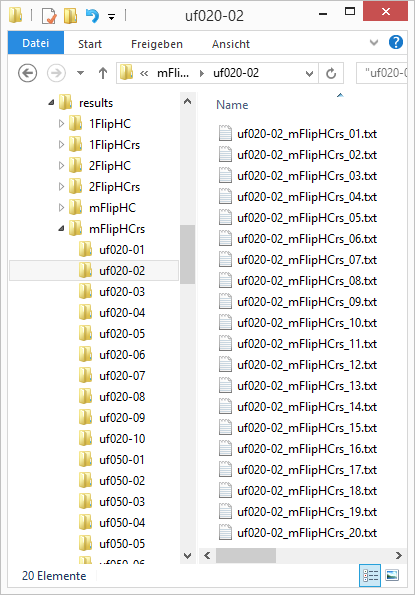
\includegraphics[width=0.33\paperwidth]{\sharedPath/graphics/optimization/sat/max3sat_example_log_file_folder_structure/max3sat_example_log_file_folder_structure}}{0.65}{0.21}%
%
\begin{locateBox}[2-5]{0.65}{0.21}
\begin{pgfpicture}%
\pgfpathrectangle{\pgfpoint{0pt}{0pt}}{\pgfpoint{0.33\paperwidth}{0.79\paperheight}}%
\pgfusepath{use as bounding box,clip}%
%
\pgfsetcolor{alertviolet}%
\pgfsetlinewidth{0.5pt}%
%
\only<3>{%
\pgfpathrectangle{\pgfpoint{0.05\paperwidth}{0.649\paperheight}}{\pgfpoint{0.07\paperwidth}{0.02\paperheight}}%
\pgfpathrectangle{\pgfpoint{0.05\paperwidth}{0.626\paperheight}}{\pgfpoint{0.07\paperwidth}{0.02\paperheight}}%
\pgfpathrectangle{\pgfpoint{0.05\paperwidth}{0.603\paperheight}}{\pgfpoint{0.07\paperwidth}{0.02\paperheight}}%
\pgfpathrectangle{\pgfpoint{0.05\paperwidth}{0.580\paperheight}}{\pgfpoint{0.07\paperwidth}{0.02\paperheight}}%
\pgfpathrectangle{\pgfpoint{0.05\paperwidth}{0.557\paperheight}}{\pgfpoint{0.07\paperwidth}{0.02\paperheight}}%
\pgfpathrectangle{\pgfpoint{0.05\paperwidth}{0.534\paperheight}}{\pgfpoint{0.07\paperwidth}{0.02\paperheight}}%
}%
%
\only<2>{%
\pgfpathrectangle{\pgfpoint{0.272\paperwidth}{0.21\paperheight}}{\pgfpoint{0.018\paperwidth}{0.445\paperheight}}%
\pgfpathrectangle{\pgfpoint{0.013\paperwidth}{0.17\paperheight}}{\pgfpoint{0.06\paperwidth}{0.02\paperheight}}%
}%
%
\only<4>{%
\pgfpathrectangle{\pgfpoint{0.06\paperwidth}{0.319\paperheight}}{\pgfpoint{0.06\paperwidth}{0.212\paperheight}}%
}%
%
\only<5>{%
\pgfpathrectangle{\pgfpoint{0.06\paperwidth}{0.513\paperheight}}{\pgfpoint{0.0433\paperwidth}{0.02\paperheight}}%
\pgfpathrectangle{\pgfpoint{0.06\paperwidth}{0.2958\paperheight}}{\pgfpoint{0.0433\paperwidth}{0.02\paperheight}}%
}%
%
\pgfusepath{stroke}%
%
\end{pgfpicture}%
\end{locateBox}%
\end{frame}%
%
\begin{frame}%
\frametitle{Example Results from \optimizationBenchmarking}%
\begin{itemize}%
\item In the following, I provide some examples for what our evaluator can do.%
\item<2-> First, a quick guide to download and run the example on your computer is given%
\item<3-> Then, I present some of the evaluation information generated by the Evaluator%
\item<4-> Finally, I will show \emph{how} that gets done in detail.%
\end{itemize}%
%
\locate{}{\pgfuseimage{optimizationBenchmarking_logo}}{0.725}{0.65}%
%
\end{frame}%
%
%
\begin{frame}[t,containsverbatim,fragile]
\frametitle{Quick Guide}%
%
\begin{itemize}%
\only<-2>{%
\item You can quickly download all example data and the Evaluator and run the example on your PC by executing the following code snippet.%
}%
\only<-2>{
\item<2-> System Requirements:%
\begin{itemize}%
\item Linux (for \texttt{make.sh}), Windows (for \texttt{make.bat}, tested: Win~8, should work also under Win~7)%
\item Java~1.7 (ideally a \texttt{JDK} under a \texttt{JRE} slower and higher memory consumption)%
\item \texttt{svn}%
\item optional: a \LaTeX\ installation, such as TeXLive (needed for generating pdf reports)%%
\end{itemize}%
}%
\only<3->{\item<3-> Enter (or create) a folder where you want to have everything, then execute this script via copy-paste to the terminal (it may need quite a while to run due to the downloads)}%
\only<6->{\item<5-> After the script, you will have%
\begin{itemize}%
\item a folder \texttt{results} with the log files which have been evaluated%
\item a folder \texttt{evaluation} with the configuration files and the \texttt{evaluation.xml} file defining what to do%
\item a filder \texttt{reports} with the generated reports%
\end{itemize}%
}%
%
\only<7->{%
\item<7-> But now, let's continue with the example\dots%
}%
\end{itemize}%
%
\only<4>{%
\begin{locateBox}{0.025}{0.29}
\begin{listingblock}[0.95\paperwidth]{Linux: script \texttt{make.sh} for downloading \& running the \maxSat\ example.}
\centering
\begin{scaledBox}{!}{0.3\paperheight}
\parbox{1.8\paperwidth}{%
\lstinputlisting[language=bash,columns=fullflexible,mathescape=false,breaklines=true,breakatwhitespace=false,showstringspaces=false]{\maxSatExamplePath/make.sh}
}%
\end{scaledBox}
\end{listingblock}
\end{locateBox}
}%
%
\only<5>{%
\begin{locateBox}{0.025}{0.29}
\begin{listingblock}[0.95\paperwidth]{Windows: script \texttt{make.bat} for downloading \& running the \maxSat\ example.}
\centering
\begin{scaledBox}{!}{0.3\paperheight}
\parbox{2.2\paperwidth}{%
\lstinputlisting[language=command.com,columns=fullflexible,mathescape=false,breaklines=true,breakatwhitespace=false,showstringspaces=false]{\maxSatExamplePath/make.bat}
}%
\end{scaledBox}
\end{listingblock}
\end{locateBox}
}%
%
\end{frame}
%
%
%
\begin{frame}[t]%
\frametitle{ECDF}%
\begin{itemize}%
\item We can plot the Empirical (Cumulative) Distribution Function (ECDF)\scitep{HAFR2012RPBBOBES,HS1998ELVAPAR,TH2004UAIAEEFSAFSAMS,WCTLTCMY2014BOAAOSFFTTSP} for us, which provides the fraction of runs that have found the solution for their respective problem at a given point in time.%  
\end{itemize}%
%
\locateWithCaption{2-6}{%
\strut\vbox to 0.475\paperheight{\vfil%
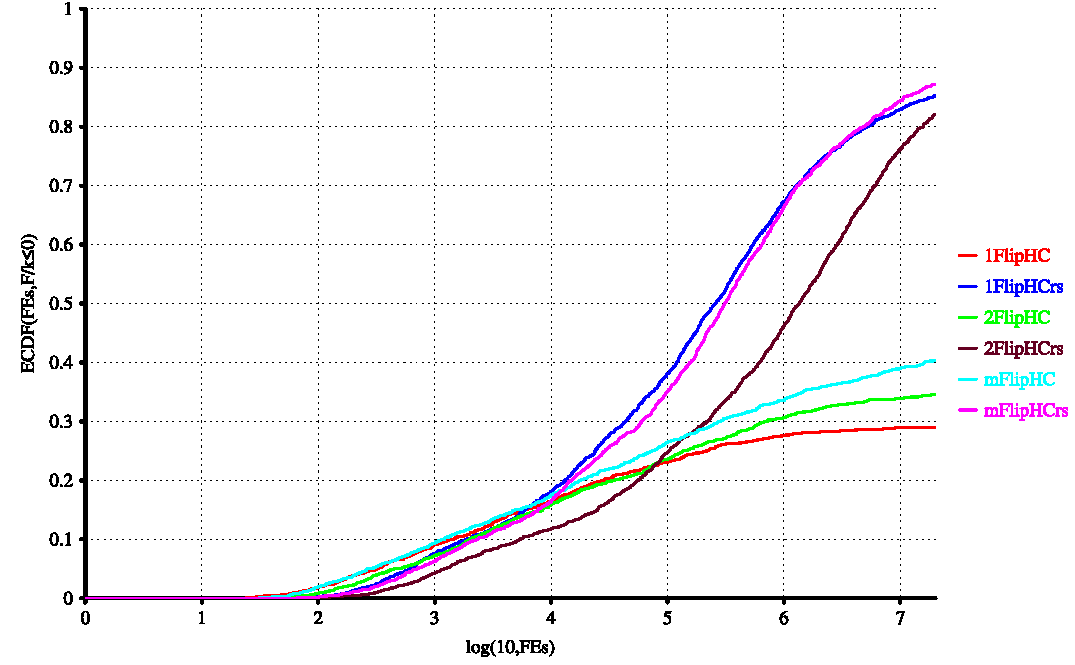
\includegraphics[scale=0.425]{\sharedPath/graphics/optimization/sat/max3sat_example_evaluation/ECDF_log_10_FEs_F_k_0/IEEEtran_ECDF_log_10_FEs_F_k_0}%
\strut\hfill\strut%
}%
}{%
The ECDF in over all 100 benchmark instances for time measure \measureFEs\ (log-scaled\only<6->{\alert{, optimized for \texttt{IEEEtran} and two figures per row}}).%
}{0.0375}{0.34}{0.925}%%
%
\locateWithCaption{7}{%
\strut\vbox to 0.475\paperheight{\vfil%
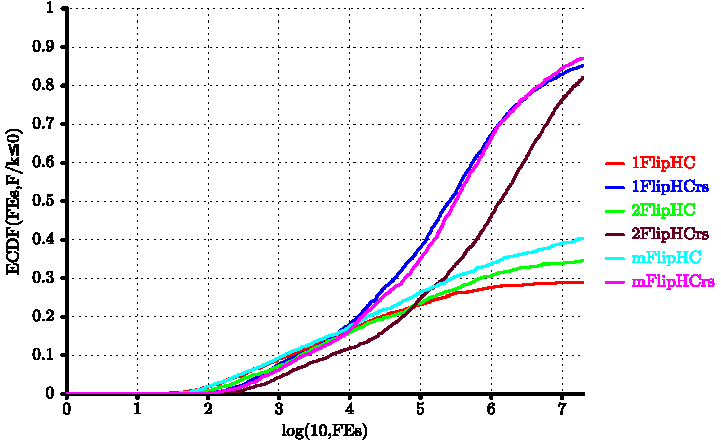
\includegraphics[scale=0.425]{\sharedPath/graphics/optimization/sat/max3sat_example_evaluation/ECDF_log_10_FEs_F_k_0/LNCS_ECDF_log_10_FEs_F_k_0}%
\strut\hfill\strut}%
}{%
The ECDF in over all 100 benchmark instances (log-scaled, \alert{optimized for \texttt{LNCS} and two figures per row}).%
}{0.0375}{0.34}{0.925}%
%
\locateWithCaption{8}{%
\strut\vbox to 0.475\paperheight{\vfil%
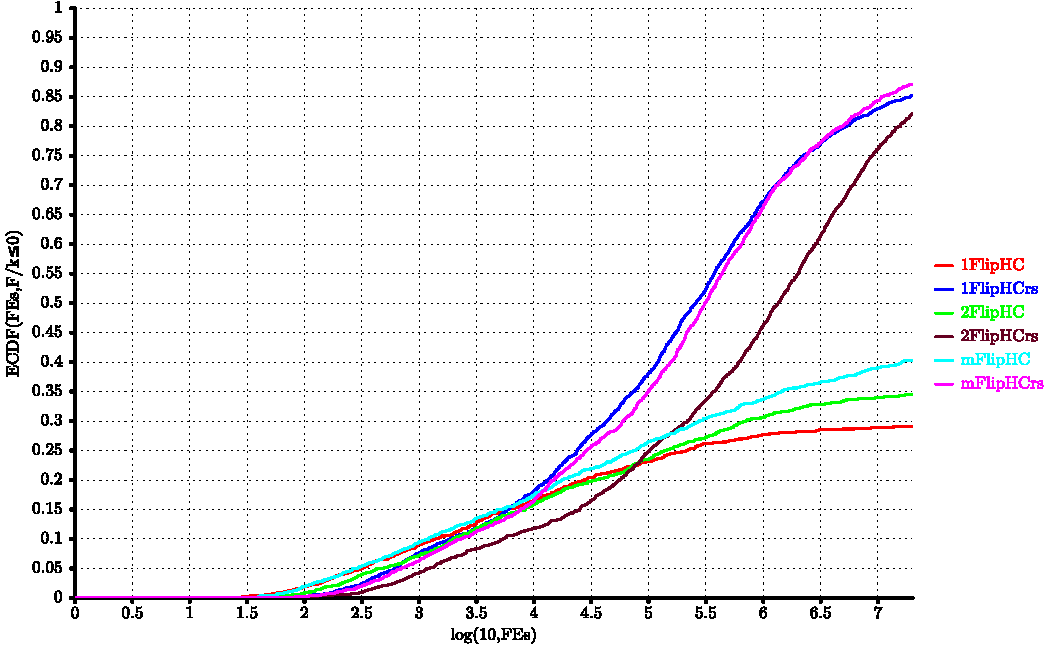
\includegraphics[scale=0.425]{\sharedPath/graphics/optimization/sat/max3sat_example_evaluation/ECDF_log_10_FEs_F_k_0/SigAlternate_ECDF_log_10_FEs_F_k_0}%
\strut\hfill\strut}%
}{%
The ECDF in over all 100 benchmark instances (log-scaled, \alert{optimized for \texttt{sig-alternate} and two figures per row}).%
}{0.0375}{0.34}{0.925}%
%
\locateWithCaption{9}{%
\strut\vbox to 0.475\paperheight{\vfil%
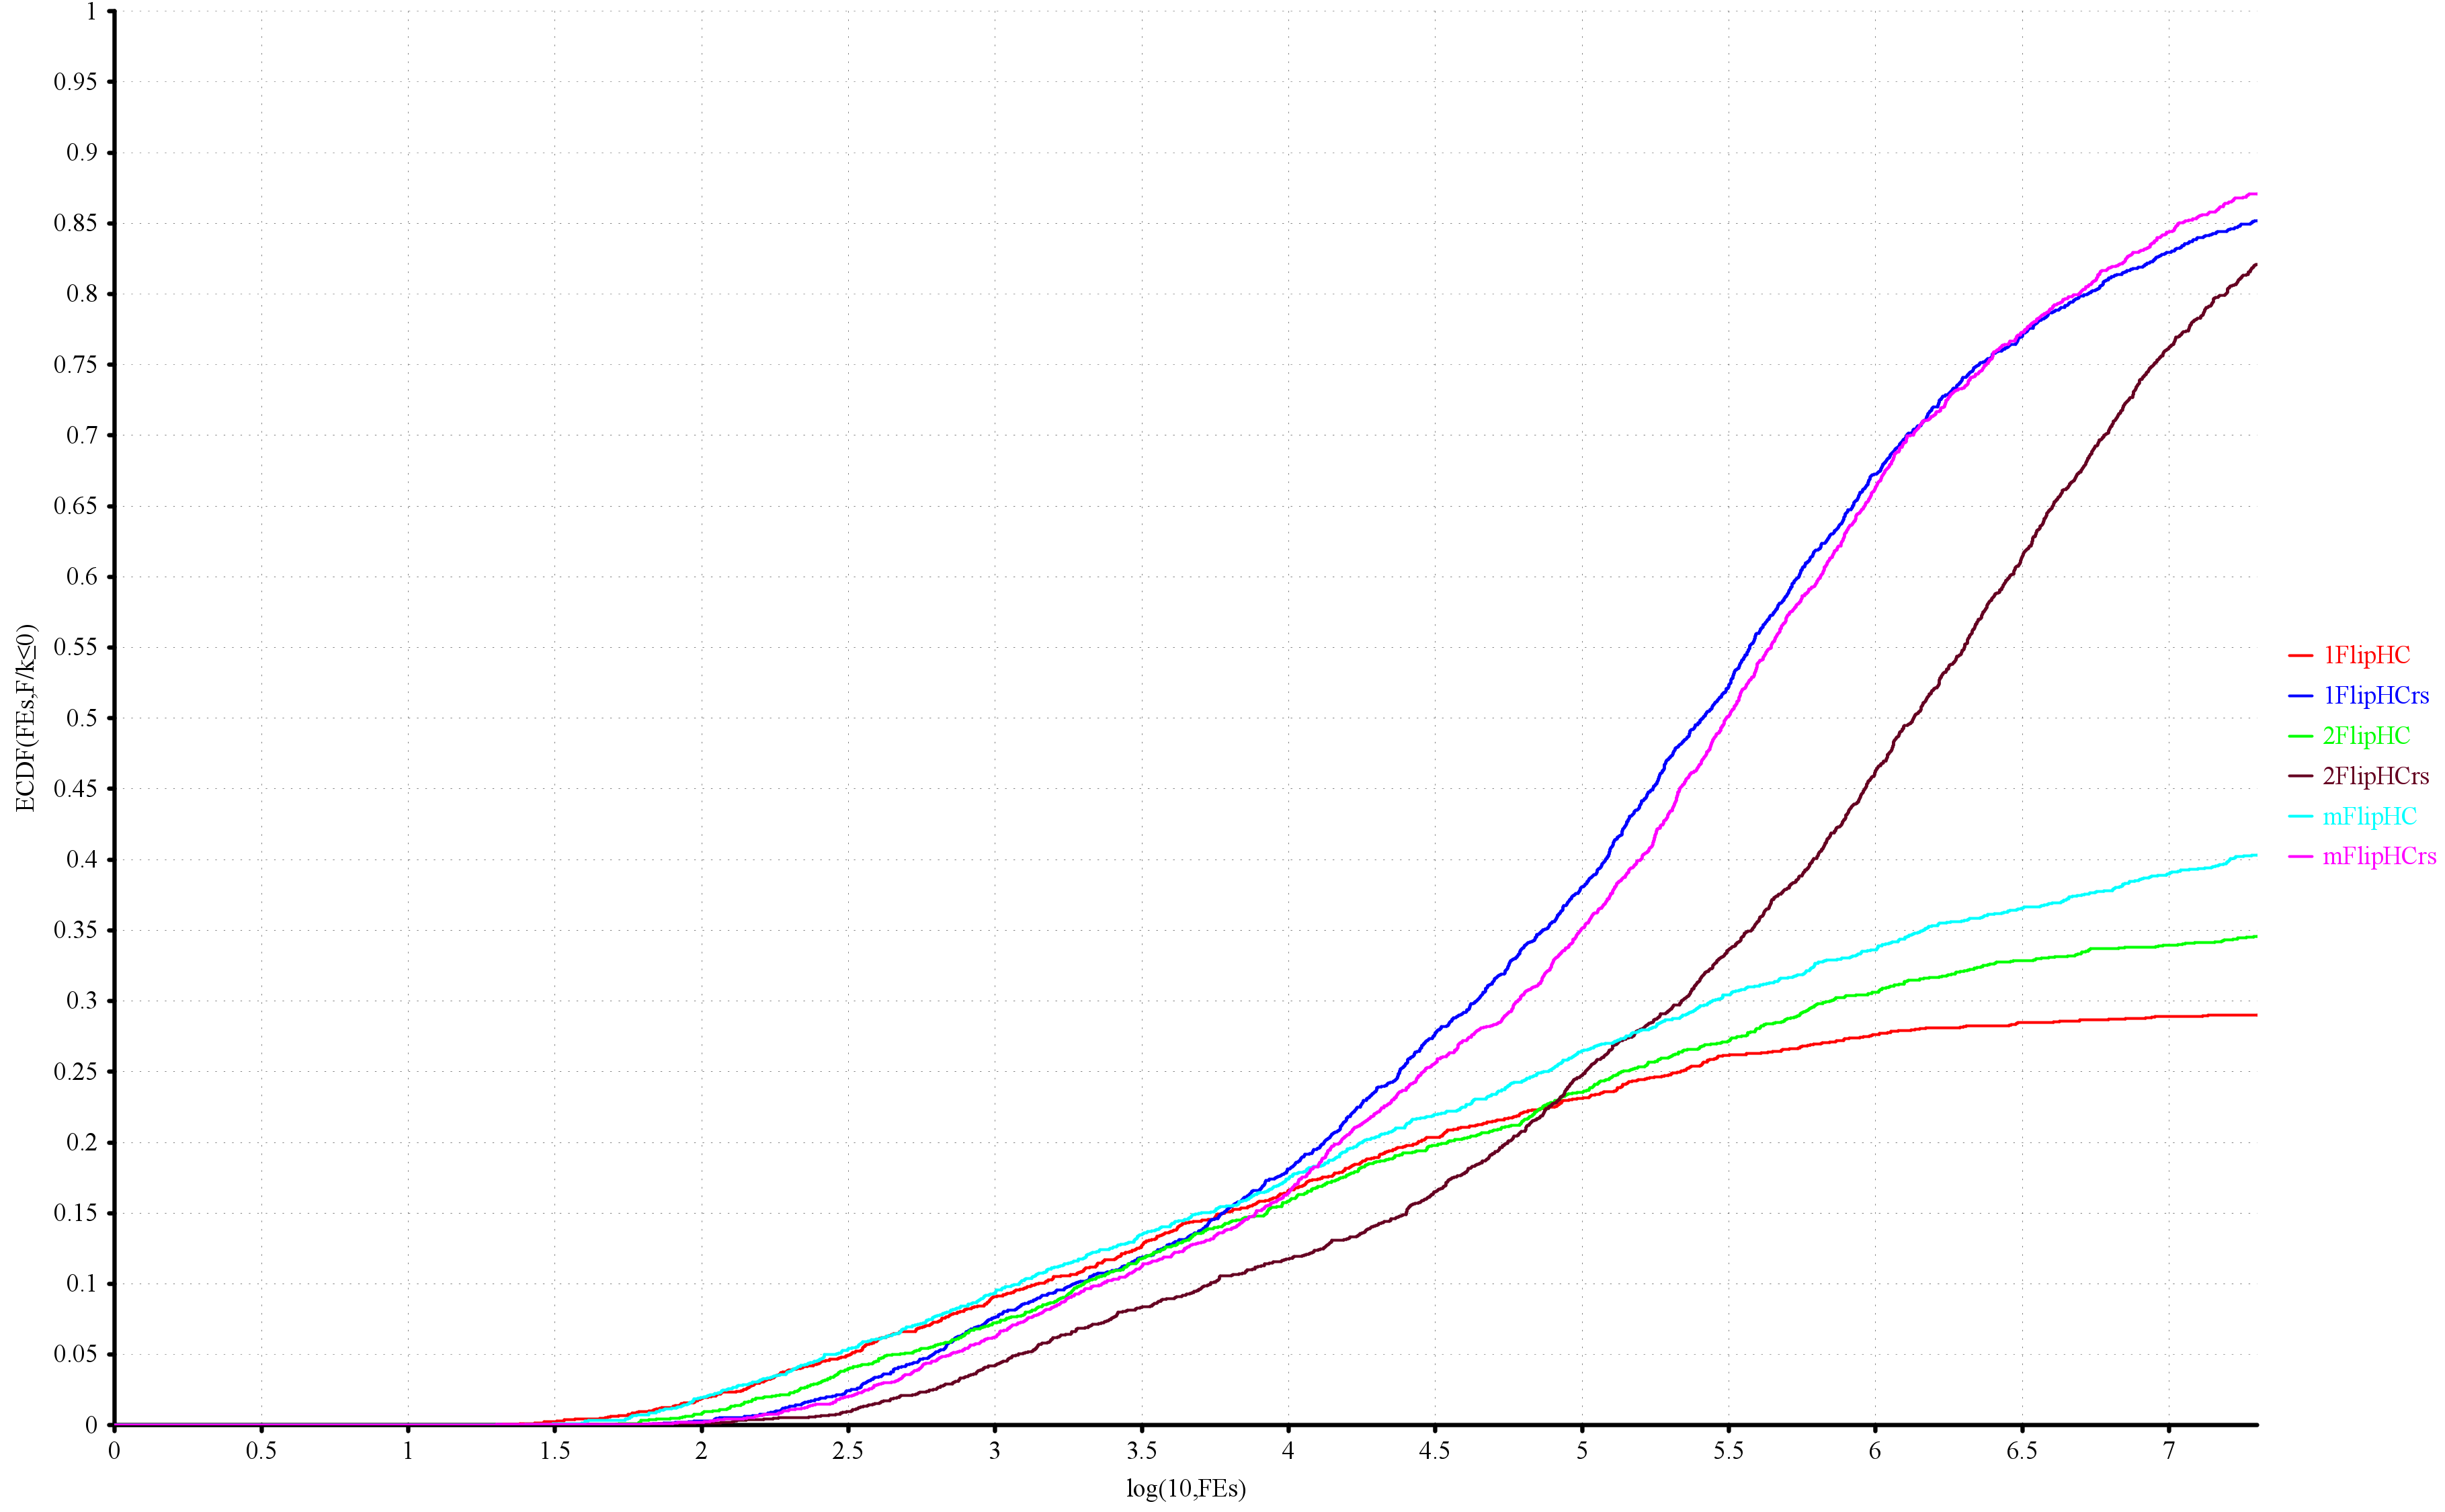
\includegraphics[width=0.6\paperwidth]{\sharedPath/graphics/optimization/sat/max3sat_example_evaluation/ECDF_log_10_FEs_F_k_0/XHTML_ECDF_log_10_FEs_F_k_0}%
\strut\hfill\strut}%
}{%
The ECDF in over all 100 benchmark instances (log-scaled, \alert{optimized for \texttt{XHTML} and two figures per row}).%
}{0.0375}{0.34}{0.925}%
%
\locate{3-}{\parbox{0.35\paperwidth}{\small%
\begin{itemize}%
\item the methods with restarts solve more problems (up to 90\%!)%
\item<4-> plain {\mFlip}s are better than {\tFlip}s are better than {\oFlip}s%
\item<5-> oddly, for restart HCers, there is a tie between the $m$- and {\oFlip} versions 
\end{itemize}%
}}{0.625}{0.3}%
%
\end{frame}%
%
\begin{frame}%
\frametitle{ECDF for Different Values of \scalebox{1.3}{\ensuremath{\mathbf{\maxSatVariables}}}}%
%
\locate{1-}{%
\parbox{0.234\paperwidth}{\raggedright\small{%
\only<-1>{We now look at the ECDF for different values of \maxSatVariables\ and a goal of 1\% unsatisfied clauses over \measureRuntime\ (log-scaled).}%
\only<2>{For $\maxSatVariables=20$, the methods with restarts are better.}%
\only<3>{But for $\maxSatVariables\geq 50$, those without reach the goal faster.}%
\only<4>{It seems that 1\% unsatisfied clauses can be reached with {\oFlip}s and without restarts.}%
\only<5>{The {\tFlip} operator again performs worst.}%
\only<6>{It looks as if it gets easier to attain a 1\% error margin if \maxSatVariables\ increases (all ECDFs reach 1).}%
\only<7-8>{For small problems, {\oFlip} is slightly faster than {\mFlip}.}%
\only<9>{For larger problems, {\mFlip} becomes slightly faster.}%
\only<10>{All in all, similar behavior over all scales (reaching 1\% error seems to be easy).}%
\only<11->{Only required runtime increases by up to 100 times.}%
}}}{0.013}{0.187}%
%
\locate{1-}{%
\parbox{0.234375\paperwidth}{\centering%
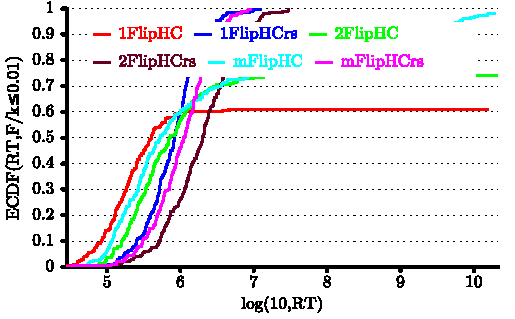
\includegraphics[width=0.234375\paperwidth]{\sharedPath/graphics/optimization/sat/max3sat_example_evaluation/ECDF_log_10_RT_F_k_0_01_distinct_n/SigAlternate_ECDF_log_10_RT_F_k_0_01_distinct_n_legend.pdf}%
\\\scriptsize{legend}}%
}{0.259375}{0.18}%
%
\locate{2-}{%
\parbox{0.234375\paperwidth}{\centering%
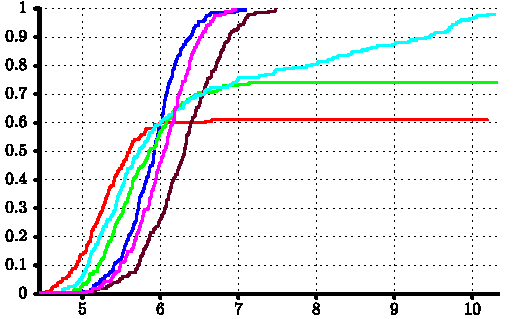
\includegraphics[width=0.234375\paperwidth]{\sharedPath/graphics/optimization/sat/max3sat_example_evaluation/ECDF_log_10_RT_F_k_0_01_distinct_n/SigAlternate_ECDF_log_10_RT_F_k_0_01_distinct_n_20.pdf}%
\\\scriptsize{$\maxSatVariables=20$}}%
}{0.50625}{0.18}%
%
\locate{3-}{%
\parbox{0.234375\paperwidth}{\centering%
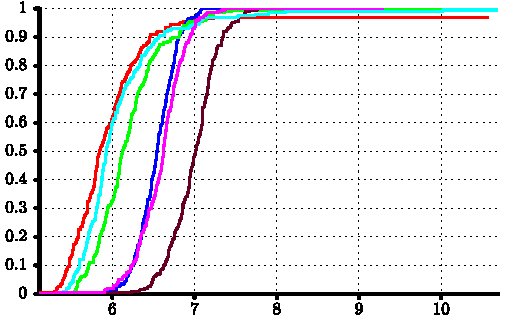
\includegraphics[width=0.234375\paperwidth]{\sharedPath/graphics/optimization/sat/max3sat_example_evaluation/ECDF_log_10_RT_F_k_0_01_distinct_n/SigAlternate_ECDF_log_10_RT_F_k_0_01_distinct_n_50.pdf}%
\\\scriptsize{$\maxSatVariables=50$}}%
}{0.753125}{0.18}%
%
\locate{4-}{%
\parbox{0.234375\paperwidth}{\centering%
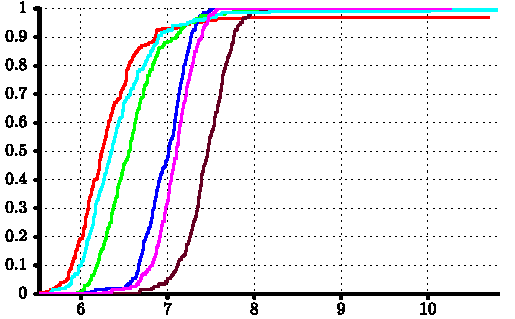
\includegraphics[width=0.234375\paperwidth]{\sharedPath/graphics/optimization/sat/max3sat_example_evaluation/ECDF_log_10_RT_F_k_0_01_distinct_n/SigAlternate_ECDF_log_10_RT_F_k_0_01_distinct_n_75.pdf}%
\\\scriptsize{$\maxSatVariables=75$}}%
}{0.0125}{0.443333333333333}%
%
\locate{5-}{%
\parbox{0.234375\paperwidth}{\centering%
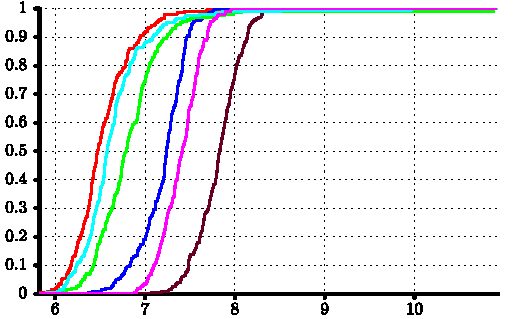
\includegraphics[width=0.234375\paperwidth]{\sharedPath/graphics/optimization/sat/max3sat_example_evaluation/ECDF_log_10_RT_F_k_0_01_distinct_n/SigAlternate_ECDF_log_10_RT_F_k_0_01_distinct_n_100.pdf}%
\\\scriptsize{$\maxSatVariables=100$}}%
}{0.259375}{0.443333333333333}%
%
\locate{6-}{%
\parbox{0.234375\paperwidth}{\centering%
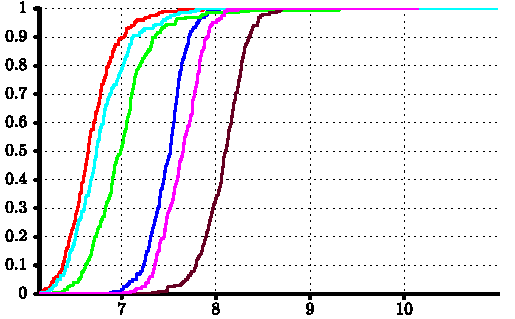
\includegraphics[width=0.234375\paperwidth]{\sharedPath/graphics/optimization/sat/max3sat_example_evaluation/ECDF_log_10_RT_F_k_0_01_distinct_n/SigAlternate_ECDF_log_10_RT_F_k_0_01_distinct_n_125.pdf}%
\\\scriptsize{$\maxSatVariables=125$}}%
}{0.50625}{0.443333333333333}%
%
\locate{7-}{%
\parbox{0.234375\paperwidth}{\centering%
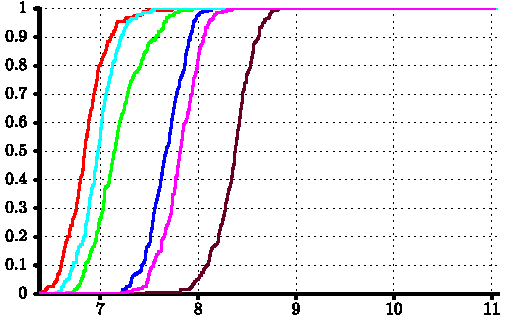
\includegraphics[width=0.234375\paperwidth]{\sharedPath/graphics/optimization/sat/max3sat_example_evaluation/ECDF_log_10_RT_F_k_0_01_distinct_n/SigAlternate_ECDF_log_10_RT_F_k_0_01_distinct_n_150.pdf}%
\\\scriptsize{$\maxSatVariables=150$}}%
}{0.753125}{0.443333333333333}%
%
\locate{8-}{%
\parbox{0.234375\paperwidth}{\centering%
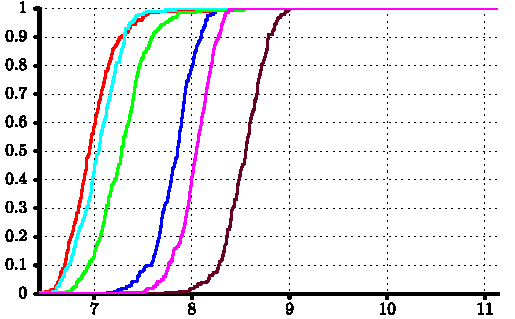
\includegraphics[width=0.234375\paperwidth]{\sharedPath/graphics/optimization/sat/max3sat_example_evaluation/ECDF_log_10_RT_F_k_0_01_distinct_n/SigAlternate_ECDF_log_10_RT_F_k_0_01_distinct_n_175.pdf}%
\\\scriptsize{$\maxSatVariables=175$}}%
}{0.0125}{0.706666666666667}%
%
\locate{9-}{%
\parbox{0.234375\paperwidth}{\centering%
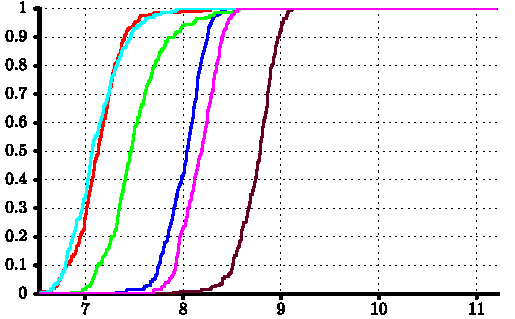
\includegraphics[width=0.234375\paperwidth]{\sharedPath/graphics/optimization/sat/max3sat_example_evaluation/ECDF_log_10_RT_F_k_0_01_distinct_n/SigAlternate_ECDF_log_10_RT_F_k_0_01_distinct_n_200.pdf}%
\\\scriptsize{$\maxSatVariables=200$}}%
}{0.259375}{0.706666666666667}%%
%
\locate{10-}{%
\parbox{0.234375\paperwidth}{\centering%
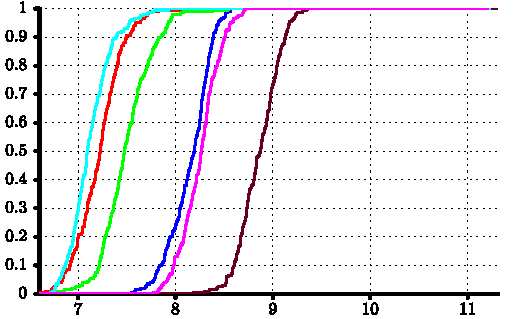
\includegraphics[width=0.234375\paperwidth]{\sharedPath/graphics/optimization/sat/max3sat_example_evaluation/ECDF_log_10_RT_F_k_0_01_distinct_n/SigAlternate_ECDF_log_10_RT_F_k_0_01_distinct_n_225.pdf}%
\\\scriptsize{$\maxSatVariables=225$}}%
}{0.50625}{0.706666666666667}%
%
\locate{11-}{%
\parbox{0.234375\paperwidth}{\centering%
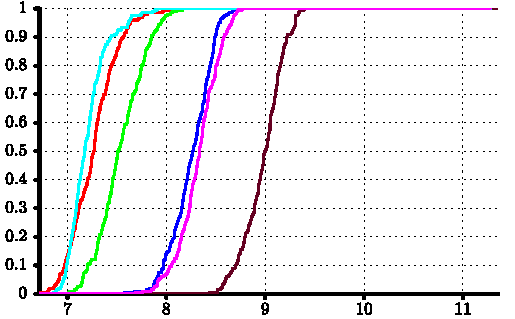
\includegraphics[width=0.234375\paperwidth]{\sharedPath/graphics/optimization/sat/max3sat_example_evaluation/ECDF_log_10_RT_F_k_0_01_distinct_n/SigAlternate_ECDF_log_10_RT_F_k_0_01_distinct_n_250.pdf}%
\\\scriptsize{$\maxSatVariables=250$}}%
}{0.753125}{0.706666666666667}%
%
\end{frame}%
%
%
\begin{frame}%
\frametitle{Progress for Different Values of \scalebox{1.3}{\ensuremath{\mathbf{\maxSatClauses}}}}%
%
\locate{1-}{%
\parbox{0.234\paperwidth}{\raggedright\small{%
\only<-1>{We now look at the progress curves (\measureObjectiveValue\ over \measureFEs\ divided by\footnote<1>{We normalize \measureFEs\ with \maxSatVariables\ in the hope to make the time measure comparable over different \maxSatVariables.} \maxSatVariables, log-scaled) for different values of \maxSatClauses.}%
\only<2>{For very small-scale problems, all algorithms behave similar.}%
\only<3>{But soon, two groups form: with and without restarts.}%
\only<4>{Algorithms using \emph{my example restart policy} seem to be slower.}%
\only<5>{The gap increases with rising \maxSatClauses}%
\only<6>{Thus, we find: algorithms with my restart policy are slower than those without\dots}%
\only<7>{{\dots}but from the ECDF we know they can solve more problems eventually.}%
\only<8>{For all scales, the initial random solutions, seem to have about 12\% of unsatisfied clauses (in median).}%
\only<9->{Convergence seems to happen between 100\maxSatVariables\ and 1000\maxSatVariables}%
}}}{0.013}{0.187}%
%
\locate{1-}{%
\parbox{0.234375\paperwidth}{\centering%
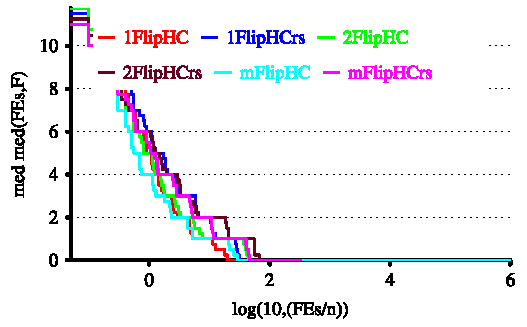
\includegraphics[width=0.234375\paperwidth]{\sharedPath/graphics/optimization/sat/max3sat_example_evaluation/med_med_log_10_FEs_n_F_distinct_k/IEEEtran_med_med_log_10_FEs_n_F_distinct_k_legend.pdf}%
\\\scriptsize{legend}}%
}{0.259375}{0.18}%
%
\locate{2-}{%
\parbox{0.234375\paperwidth}{\centering%
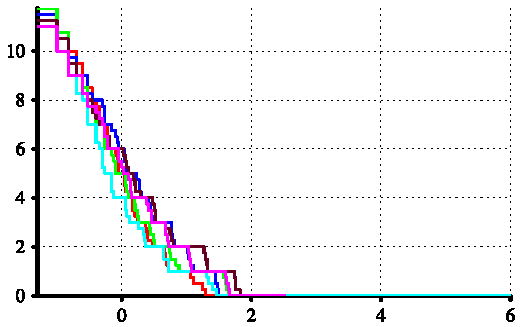
\includegraphics[width=0.234375\paperwidth]{\sharedPath/graphics/optimization/sat/max3sat_example_evaluation/med_med_log_10_FEs_n_F_distinct_k/IEEEtran_med_med_log_10_FEs_n_F_distinct_k_91.pdf}%
\\\scriptsize{$\maxSatClauses=91$}}%
}{0.50625}{0.18}%
%
\locate{3-}{%
\parbox{0.234375\paperwidth}{\centering%
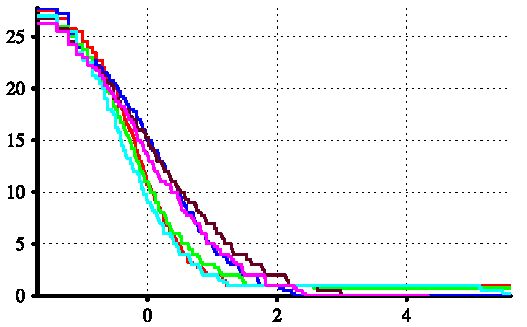
\includegraphics[width=0.234375\paperwidth]{\sharedPath/graphics/optimization/sat/max3sat_example_evaluation/med_med_log_10_FEs_n_F_distinct_k/IEEEtran_med_med_log_10_FEs_n_F_distinct_k_218.pdf}%
\\\scriptsize{$\maxSatClauses=218$}}%
}{0.753125}{0.18}%
%
\locate{4-}{%
\parbox{0.234375\paperwidth}{\centering%
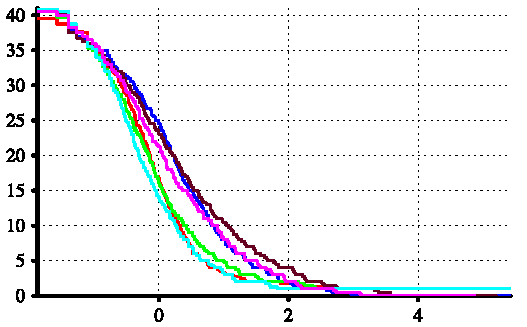
\includegraphics[width=0.234375\paperwidth]{\sharedPath/graphics/optimization/sat/max3sat_example_evaluation/med_med_log_10_FEs_n_F_distinct_k/IEEEtran_med_med_log_10_FEs_n_F_distinct_k_325.pdf}%
\\\scriptsize{$\maxSatClauses=325$}}%
}{0.0125}{0.443333333333333}%
%
\locate{5-}{%
\parbox{0.234375\paperwidth}{\centering%
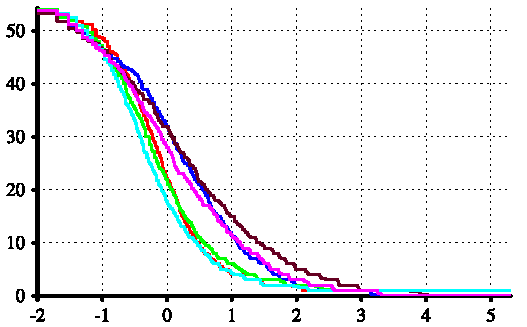
\includegraphics[width=0.234375\paperwidth]{\sharedPath/graphics/optimization/sat/max3sat_example_evaluation/med_med_log_10_FEs_n_F_distinct_k/IEEEtran_med_med_log_10_FEs_n_F_distinct_k_430.pdf}%
\\\scriptsize{$\maxSatClauses=430$}}%
}{0.259375}{0.443333333333333}%
%
\locate{6-}{%
\parbox{0.234375\paperwidth}{\centering%
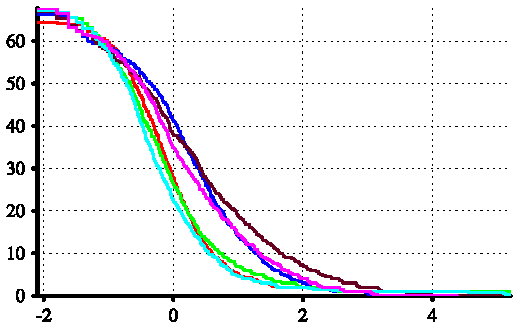
\includegraphics[width=0.234375\paperwidth]{\sharedPath/graphics/optimization/sat/max3sat_example_evaluation/med_med_log_10_FEs_n_F_distinct_k/IEEEtran_med_med_log_10_FEs_n_F_distinct_k_538.pdf}%
\\\scriptsize{$\maxSatClauses=538$}}%
}{0.50625}{0.443333333333333}%
%
\locate{7-}{%
\parbox{0.234375\paperwidth}{\centering%
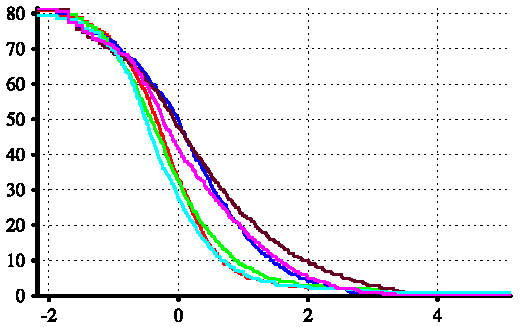
\includegraphics[width=0.234375\paperwidth]{\sharedPath/graphics/optimization/sat/max3sat_example_evaluation/med_med_log_10_FEs_n_F_distinct_k/IEEEtran_med_med_log_10_FEs_n_F_distinct_k_645.pdf}%
\\\scriptsize{$\maxSatClauses=645$}}%
}{0.753125}{0.443333333333333}%
%
\locate{8-}{%
\parbox{0.234375\paperwidth}{\centering%
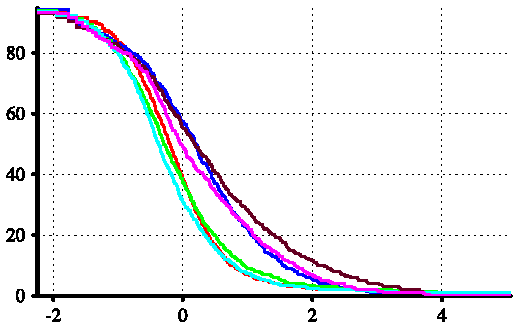
\includegraphics[width=0.234375\paperwidth]{\sharedPath/graphics/optimization/sat/max3sat_example_evaluation/med_med_log_10_FEs_n_F_distinct_k/IEEEtran_med_med_log_10_FEs_n_F_distinct_k_753.pdf}%
\\\scriptsize{$\maxSatClauses=753$}}%
}{0.0125}{0.706666666666667}%
%
\locate{9-}{%
\parbox{0.234375\paperwidth}{\centering%
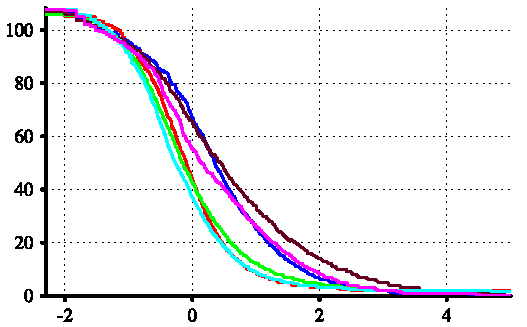
\includegraphics[width=0.234375\paperwidth]{\sharedPath/graphics/optimization/sat/max3sat_example_evaluation/med_med_log_10_FEs_n_F_distinct_k/IEEEtran_med_med_log_10_FEs_n_F_distinct_k_860.pdf}%
\\\scriptsize{$\maxSatClauses=860$}}%
}{0.259375}{0.706666666666667}%%
%
\locate{10-}{%
\parbox{0.234375\paperwidth}{\centering%
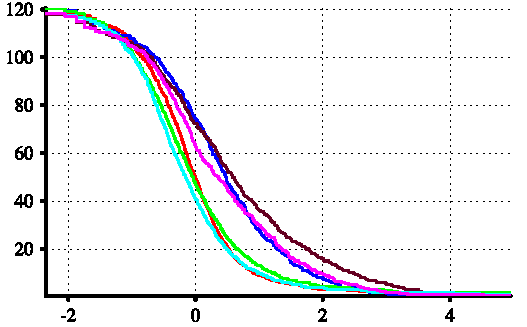
\includegraphics[width=0.234375\paperwidth]{\sharedPath/graphics/optimization/sat/max3sat_example_evaluation/med_med_log_10_FEs_n_F_distinct_k/IEEEtran_med_med_log_10_FEs_n_F_distinct_k_960.pdf}%
\\\scriptsize{$\maxSatClauses=960$}}%
}{0.50625}{0.706666666666667}%
%
\locate{11-}{%
\parbox{0.234375\paperwidth}{\centering%
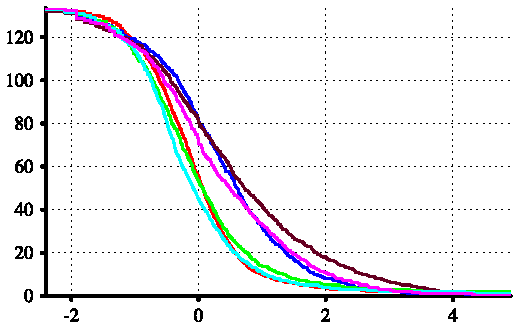
\includegraphics[width=0.234375\paperwidth]{\sharedPath/graphics/optimization/sat/max3sat_example_evaluation/med_med_log_10_FEs_n_F_distinct_k/IEEEtran_med_med_log_10_FEs_n_F_distinct_k_1065.pdf}%
\\\scriptsize{$\maxSatClauses=1065$}}%
}{0.753125}{0.706666666666667}%
%
\end{frame}%
%
%
\begin{frame}%
\frametitle{StdDev of \measureObjectiveValue\ for Different Values of \scalebox{1.3}{\ensuremath{\mathbf{\maxSatVariables}}}}%
%
\locate{1-}{%
\parbox{0.234\paperwidth}{\raggedright\small{%
\only<-1>{Let's look at the standard deviation of the best objective value \measureObjectiveValue\ (divided by\footnote<1>{Since \measureObjectiveValue\ is always in $1\dots\maxSatClauses$, dividing it by \maxSatClauses\ normalizes it into $[0,1]$ and makes the values comparable for different \maxSatClauses\ or \maxSatVariables.} \maxSatClauses) found over \measureRuntime\ (log-scaled) for different values of \maxSatVariables.}%
\only<2>{For small-scale problems, the standard deviation seems to decrease steadily.}%
\only<3>{The reason is probably that the algorithms converge nicely.}%
\only<4>{For the methods with restarts, it reaches very close to 0.}%
\only<5>{For those without, it remains constant above 0 after some time.}%
\only<6>{These algorithms probably get stuck at different local optima in different runs.}%
\only<7>{For increasing scales, the standard deviation goes first down, then up, then farther down.}%
\only<8>{Maybe there is some kind of hard-to-attain improvement that some runs find earlier than others.}%
\only<9>{The time of convergence seems to increase for the methods with restarts with \maxSatVariables.}%
\only<10->{The early standard deviations are usually below 0.03 and highest for small \maxSatVariables.}% 
}}}{0.013}{0.187}%
%
\locate{1-}{%
\parbox{0.234375\paperwidth}{\centering%
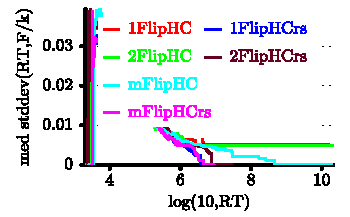
\includegraphics[width=0.234375\paperwidth]{\sharedPath/graphics/optimization/sat/max3sat_example_evaluation/med_stddev_log_10_RT_F_k_distinct_n/LNCS_med_stddev_log_10_RT_F_k_distinct_n_legend.pdf}%
\\\scriptsize{legend}}%
}{0.259375}{0.18}%
%
\locate{2-}{%
\parbox{0.234375\paperwidth}{\centering%
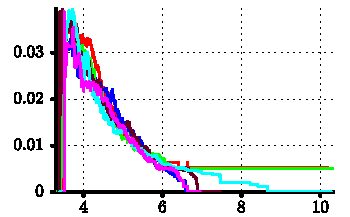
\includegraphics[width=0.234375\paperwidth]{\sharedPath/graphics/optimization/sat/max3sat_example_evaluation/med_stddev_log_10_RT_F_k_distinct_n/LNCS_med_stddev_log_10_RT_F_k_distinct_n_20.pdf}%
\\\scriptsize{$\maxSatVariables=20$}}%
}{0.50625}{0.18}%
%
\locate{3-}{%
\parbox{0.234375\paperwidth}{\centering%
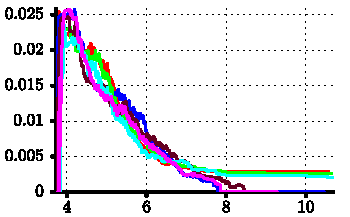
\includegraphics[width=0.234375\paperwidth]{\sharedPath/graphics/optimization/sat/max3sat_example_evaluation/med_stddev_log_10_RT_F_k_distinct_n/LNCS_med_stddev_log_10_RT_F_k_distinct_n_50.pdf}%
\\\scriptsize{$\maxSatVariables=50$}}%
}{0.753125}{0.18}%
%
\locate{4-}{%
\parbox{0.234375\paperwidth}{\centering%
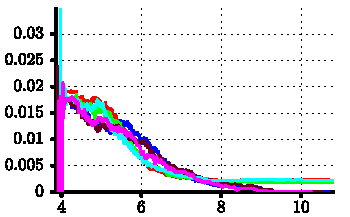
\includegraphics[width=0.234375\paperwidth]{\sharedPath/graphics/optimization/sat/max3sat_example_evaluation/med_stddev_log_10_RT_F_k_distinct_n/LNCS_med_stddev_log_10_RT_F_k_distinct_n_75.pdf}%
\\\scriptsize{$\maxSatVariables=75$}}%
}{0.0125}{0.443333333333333}%
%
\locate{5-}{%
\parbox{0.234375\paperwidth}{\centering%
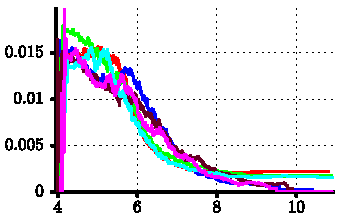
\includegraphics[width=0.234375\paperwidth]{\sharedPath/graphics/optimization/sat/max3sat_example_evaluation/med_stddev_log_10_RT_F_k_distinct_n/LNCS_med_stddev_log_10_RT_F_k_distinct_n_100.pdf}%
\\\scriptsize{$\maxSatVariables=100$}}%
}{0.259375}{0.443333333333333}%
%
\locate{6-}{%
\parbox{0.234375\paperwidth}{\centering%
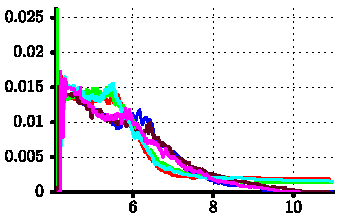
\includegraphics[width=0.234375\paperwidth]{\sharedPath/graphics/optimization/sat/max3sat_example_evaluation/med_stddev_log_10_RT_F_k_distinct_n/LNCS_med_stddev_log_10_RT_F_k_distinct_n_125.pdf}%
\\\scriptsize{$\maxSatVariables=125$}}%
}{0.50625}{0.443333333333333}%
%
\locate{7-}{%
\parbox{0.234375\paperwidth}{\centering%
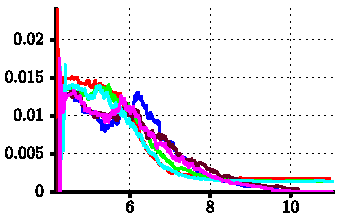
\includegraphics[width=0.234375\paperwidth]{\sharedPath/graphics/optimization/sat/max3sat_example_evaluation/med_stddev_log_10_RT_F_k_distinct_n/LNCS_med_stddev_log_10_RT_F_k_distinct_n_150.pdf}%
\\\scriptsize{$\maxSatVariables=150$}}%
}{0.753125}{0.443333333333333}%
%
\locate{8-}{%
\parbox{0.234375\paperwidth}{\centering%
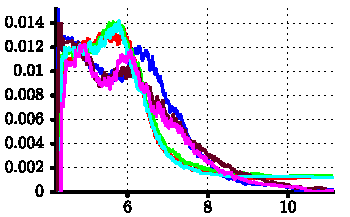
\includegraphics[width=0.234375\paperwidth]{\sharedPath/graphics/optimization/sat/max3sat_example_evaluation/med_stddev_log_10_RT_F_k_distinct_n/LNCS_med_stddev_log_10_RT_F_k_distinct_n_175.pdf}%
\\\scriptsize{$\maxSatVariables=175$}}%
}{0.0125}{0.706666666666667}%
%
\locate{9-}{%
\parbox{0.234375\paperwidth}{\centering%
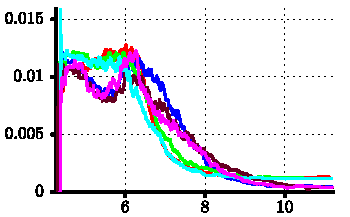
\includegraphics[width=0.234375\paperwidth]{\sharedPath/graphics/optimization/sat/max3sat_example_evaluation/med_stddev_log_10_RT_F_k_distinct_n/LNCS_med_stddev_log_10_RT_F_k_distinct_n_200.pdf}%
\\\scriptsize{$\maxSatVariables=200$}}%
}{0.259375}{0.706666666666667}%%
%
\locate{10-}{%
\parbox{0.234375\paperwidth}{\centering%
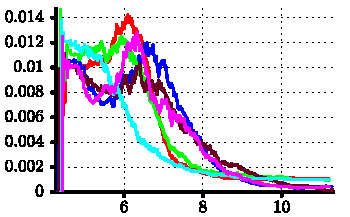
\includegraphics[width=0.234375\paperwidth]{\sharedPath/graphics/optimization/sat/max3sat_example_evaluation/med_stddev_log_10_RT_F_k_distinct_n/LNCS_med_stddev_log_10_RT_F_k_distinct_n_225.pdf}%
\\\scriptsize{$\maxSatVariables=225$}}%
}{0.50625}{0.706666666666667}%
%
\locate{11-}{%
\parbox{0.234375\paperwidth}{\centering%
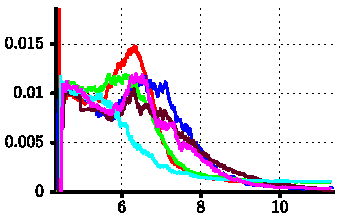
\includegraphics[width=0.234375\paperwidth]{\sharedPath/graphics/optimization/sat/max3sat_example_evaluation/med_stddev_log_10_RT_F_k_distinct_n/LNCS_med_stddev_log_10_RT_F_k_distinct_n_250.pdf}%
\\\scriptsize{$\maxSatVariables=250$}}%
}{0.753125}{0.706666666666667}%
%
\end{frame}%
%
%
\begin{frame}%
\frametitle{So{\dots} how to get there?}%
\begin{itemize}%
\item So these are \emph{some} of the things \optimizationBenchmarking\ can \emph{currently} do.%
\item<2-> But how to do them?\\\strut\\\strut\\\strut%
\end{itemize}%
\locate{}{\pgfuseimage{optimizationBenchmarking_logo}}{0.725}{0.65}%
\end{frame}%
%
\begin{frame}%
\frametitle{The Flow}%
\begin{itemize}%
\item Let us now take a closer look on how the \optimizationBenchmarking\ evaluator is used (and works)%
\end{itemize}%
\end{frame}%
%
\begin{frame}[b]%
\frametitle{The Flow}%
%
\locate{1-2}{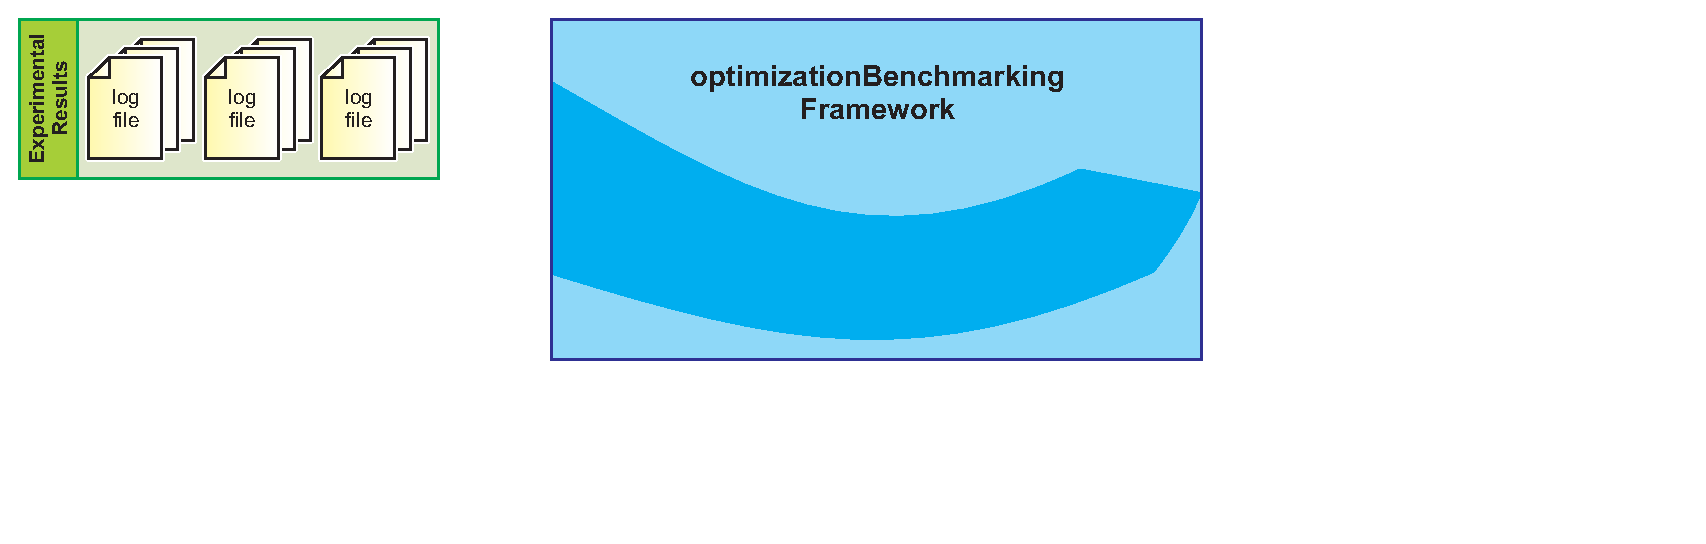
\includegraphics[width=0.9\paperwidth]{\sharedPath/graphics/optimizationBenchmarking/optimizationBenchmarking_flow/optimizationBenchmarking_flow_input_1_results}}{0.05}{0.16}%
\locate{3-4}{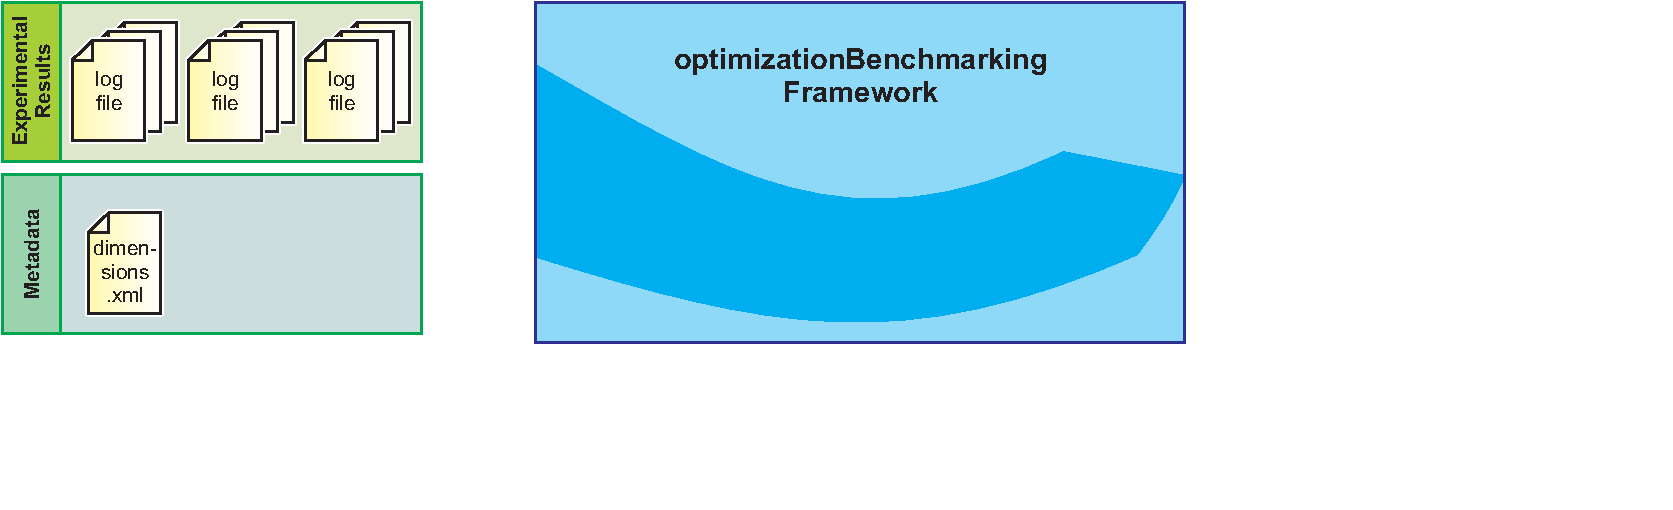
\includegraphics[width=0.9\paperwidth]{\sharedPath/graphics/optimizationBenchmarking/optimizationBenchmarking_flow/optimizationBenchmarking_flow_input_2_dimensions}}{0.05}{0.16}%
\locate{5-6}{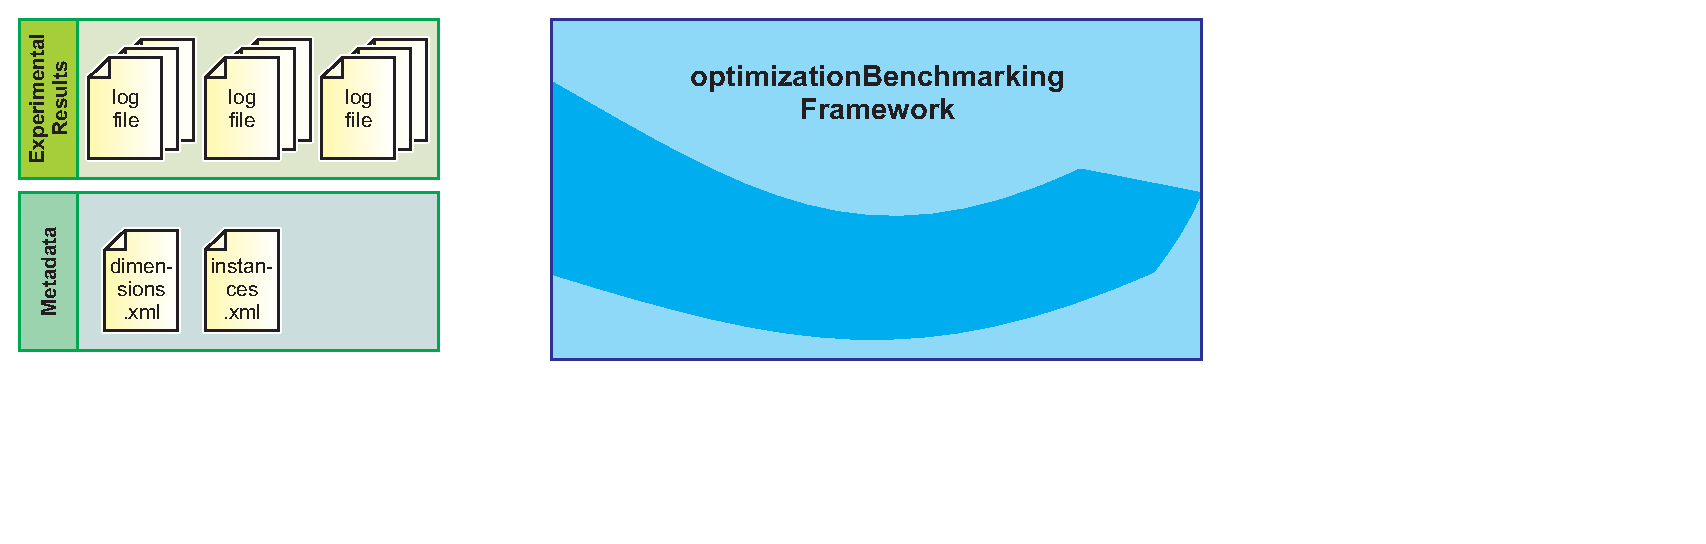
\includegraphics[width=0.9\paperwidth]{\sharedPath/graphics/optimizationBenchmarking/optimizationBenchmarking_flow/optimizationBenchmarking_flow_input_3_instances}}{0.05}{0.16}%
\locate{7-8}{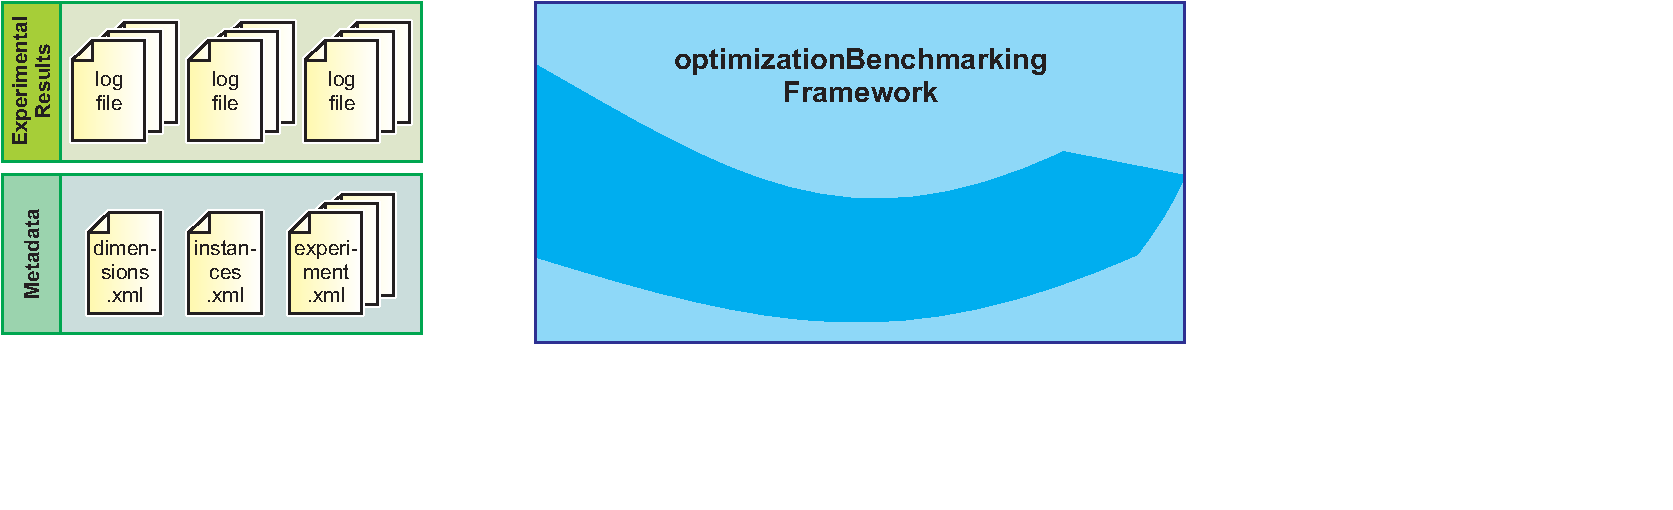
\includegraphics[width=0.9\paperwidth]{\sharedPath/graphics/optimizationBenchmarking/optimizationBenchmarking_flow/optimizationBenchmarking_flow_input_4_experiment}}{0.05}{0.16}%
\locate{9-10}{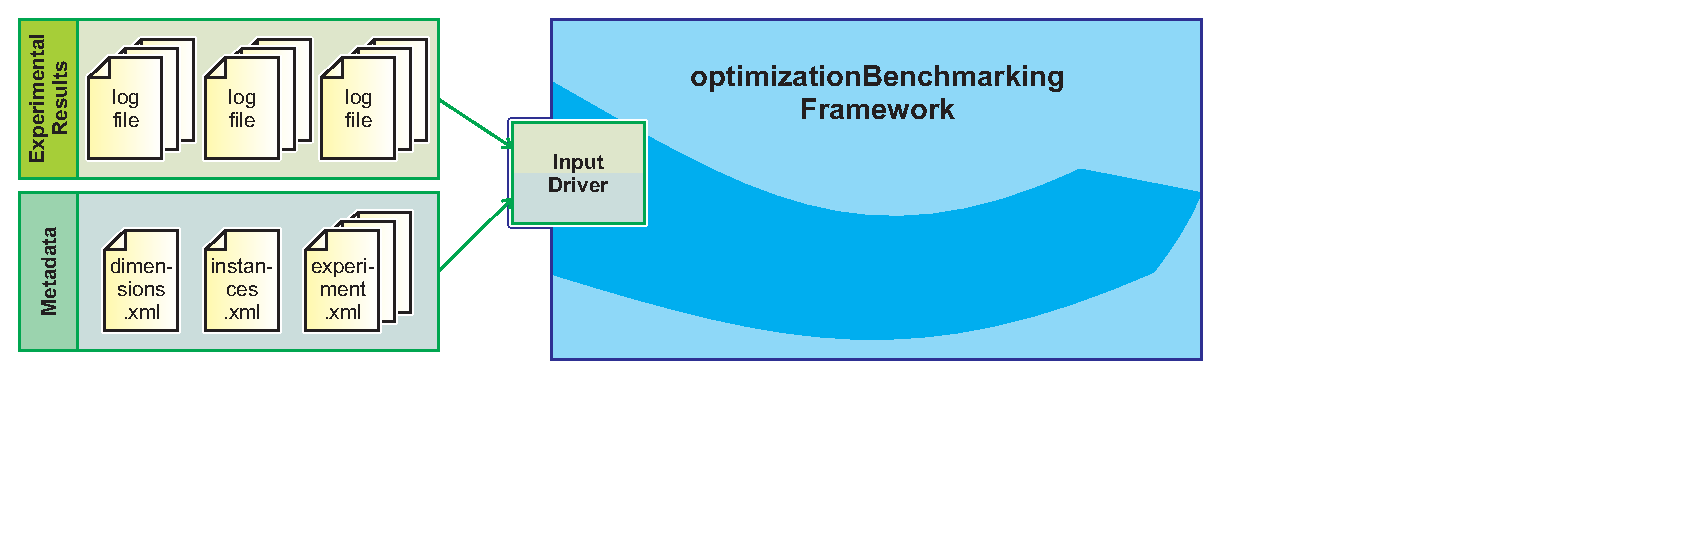
\includegraphics[width=0.9\paperwidth]{\sharedPath/graphics/optimizationBenchmarking/optimizationBenchmarking_flow/optimizationBenchmarking_flow_input_5_driver}}{0.05}{0.16}%
\locate{11}{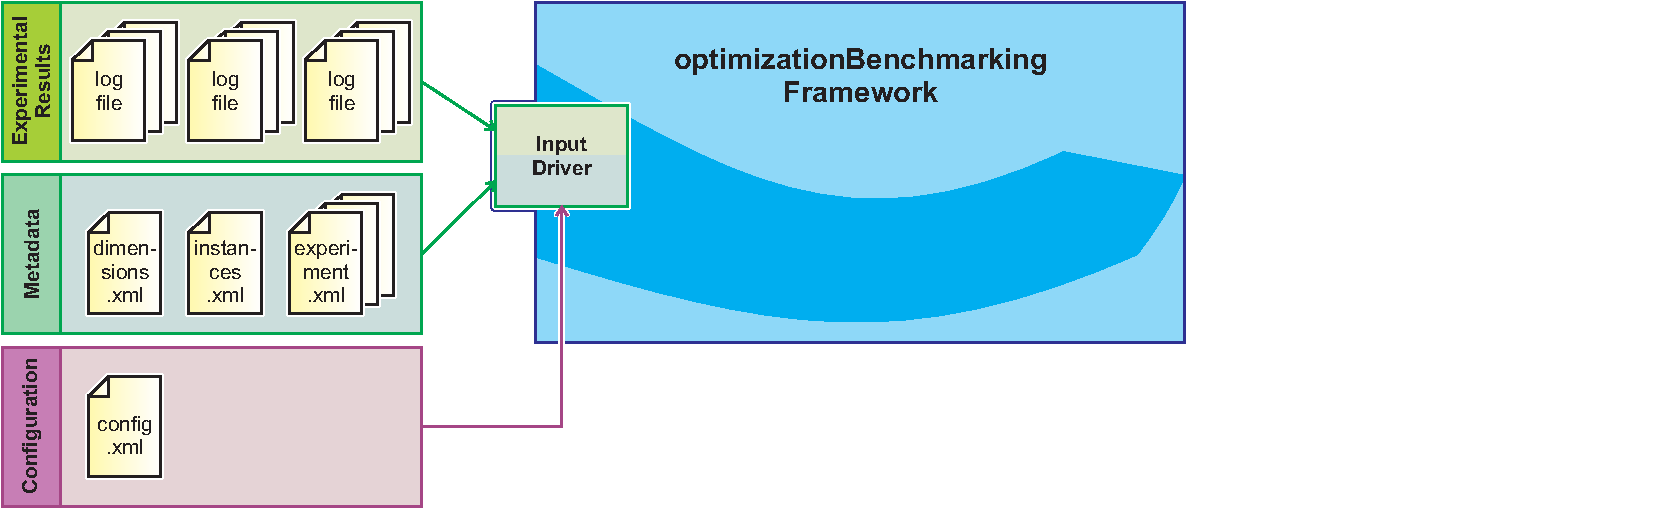
\includegraphics[width=0.9\paperwidth]{\sharedPath/graphics/optimizationBenchmarking/optimizationBenchmarking_flow/optimizationBenchmarking_flow_config_1_config}}{0.05}{0.16}%
\locate{12}{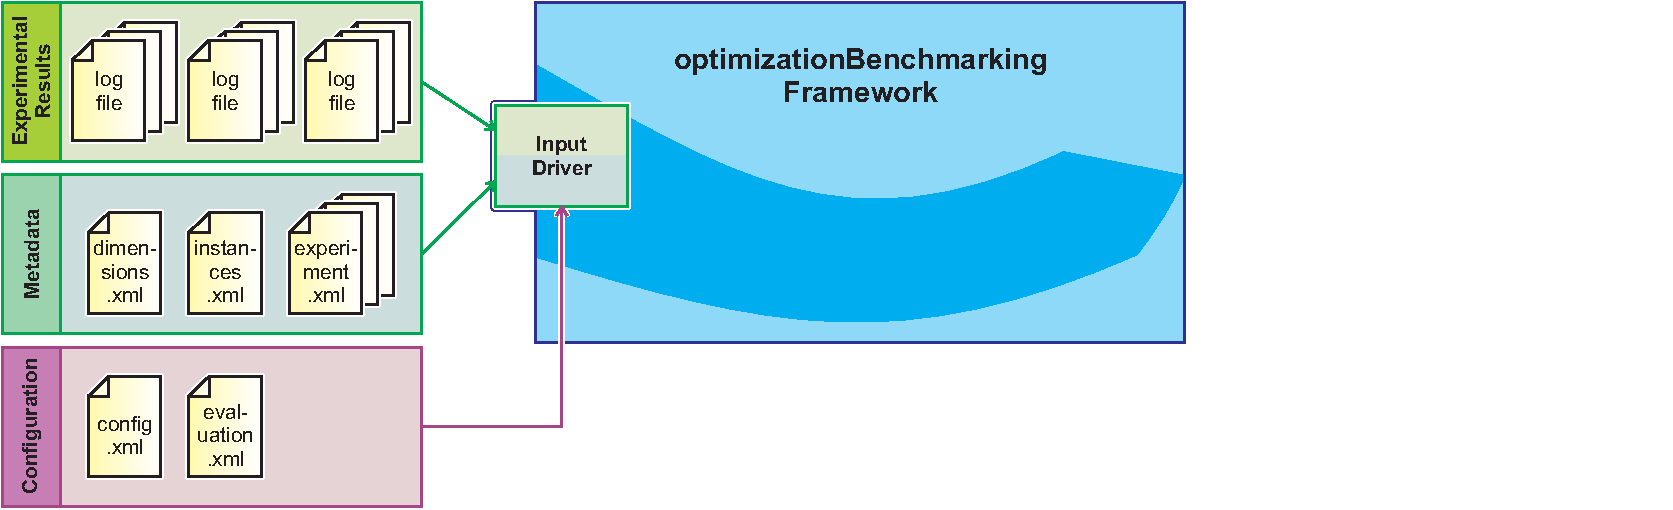
\includegraphics[width=0.9\paperwidth]{\sharedPath/graphics/optimizationBenchmarking/optimizationBenchmarking_flow/optimizationBenchmarking_flow_config_2_evaluation}}{0.05}{0.16}%
\locate{13-14}{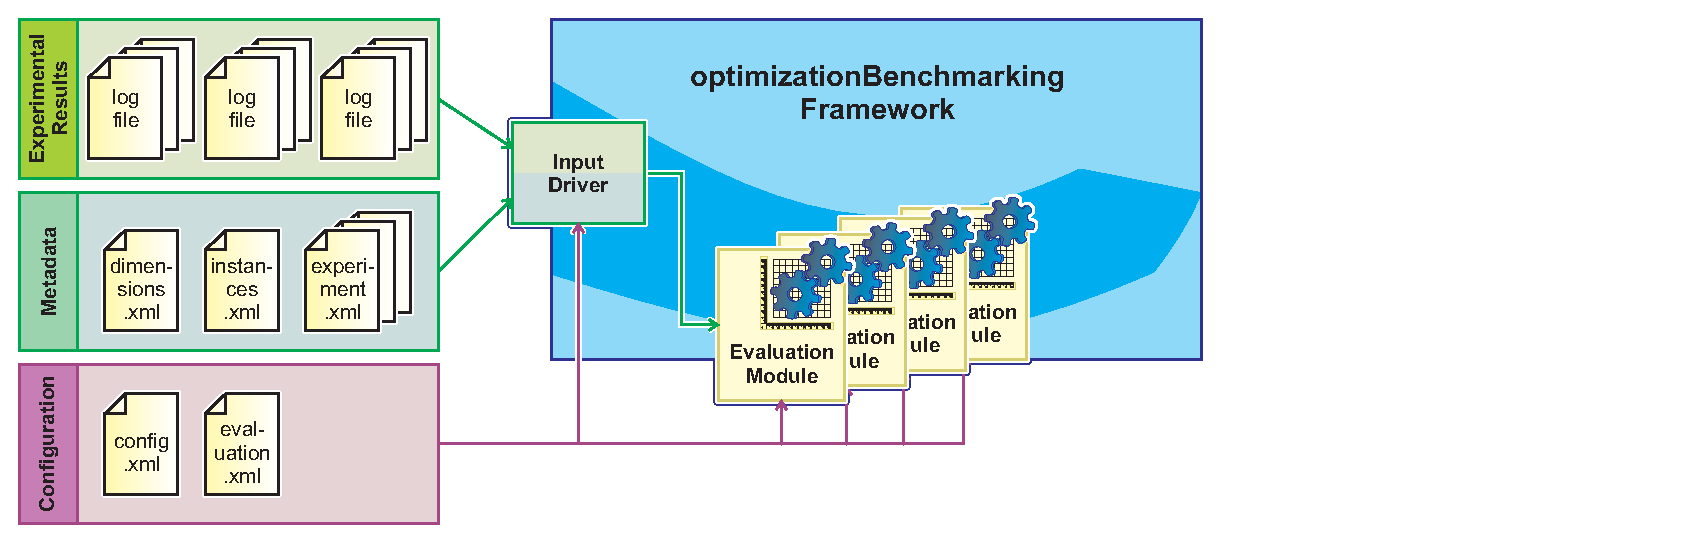
\includegraphics[width=0.9\paperwidth]{\sharedPath/graphics/optimizationBenchmarking/optimizationBenchmarking_flow/optimizationBenchmarking_flow_evaluation}}{0.05}{0.16}%
\locate{15}{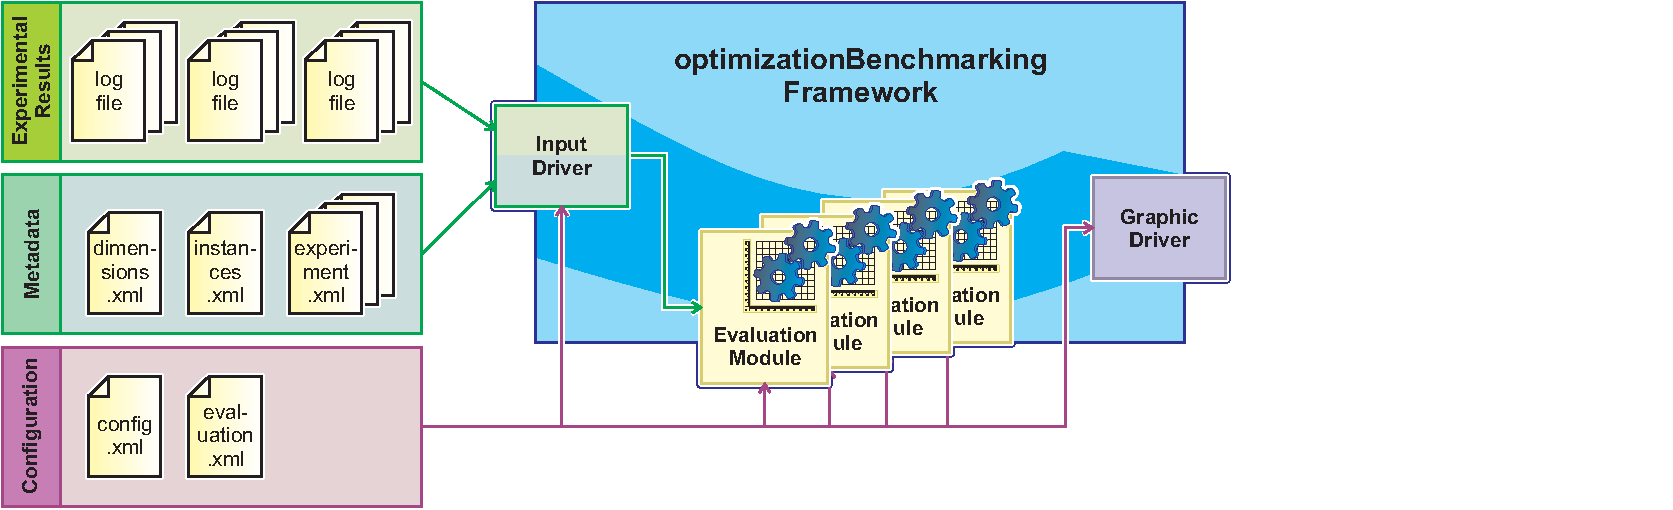
\includegraphics[width=0.9\paperwidth]{\sharedPath/graphics/optimizationBenchmarking/optimizationBenchmarking_flow/optimizationBenchmarking_flow_output_1_graphic}}{0.05}{0.16}%
\locate{16}{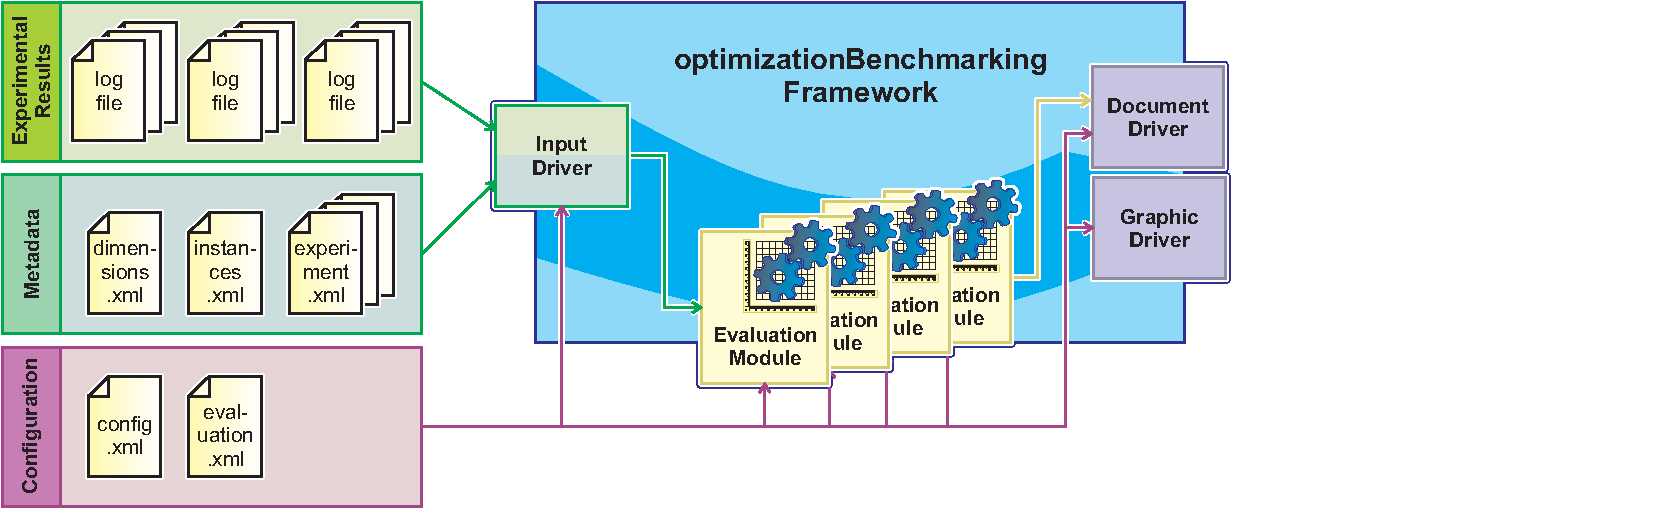
\includegraphics[width=0.9\paperwidth]{\sharedPath/graphics/optimizationBenchmarking/optimizationBenchmarking_flow/optimizationBenchmarking_flow_output_2_document}}{0.05}{0.16}%
\locate{17}{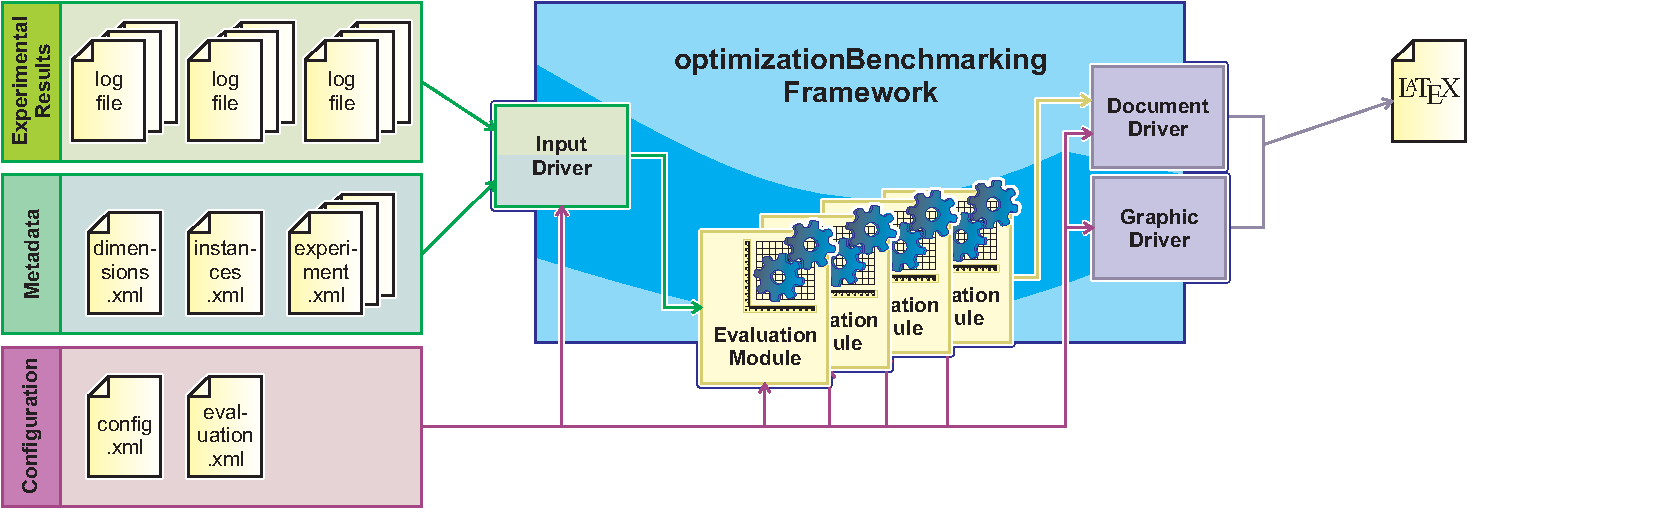
\includegraphics[width=0.9\paperwidth]{\sharedPath/graphics/optimizationBenchmarking/optimizationBenchmarking_flow/optimizationBenchmarking_flow_output_3_latex}}{0.05}{0.16}%
\locate{18-20}{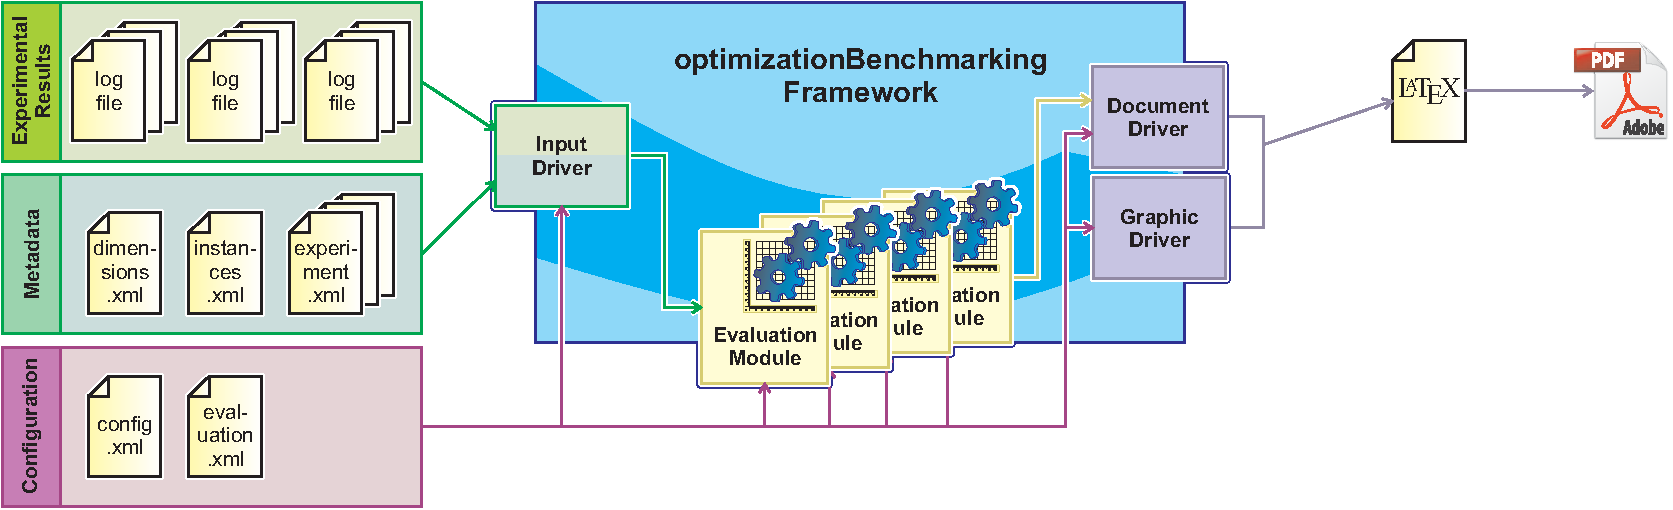
\includegraphics[width=0.9\paperwidth]{\sharedPath/graphics/optimizationBenchmarking/optimizationBenchmarking_flow/optimizationBenchmarking_flow_output_4_pdf}}{0.05}{0.16}%
\locate{21}{\includegraphics[width=0.9\paperwidth]{\sharedPath/graphics/optimizationBenchmarking/optimizationBenchmarking_flow/optimizationBenchmarking_flow_output_5_xhtml}}{0.05}{0.16}%
\locate{22-}{\includegraphics[width=0.9\paperwidth]{\sharedPath/graphics/optimizationBenchmarking/optimizationBenchmarking_flow/optimizationBenchmarking_flow}}{0.05}{0.16}%
%
\begin{small}%
\begin{itemize}%
%
\only<-8>{%
\item We got a couple of log files for each experiment\uncover<2->{: 6 experiments in our example, each with $10\times 10\times 20=\numprint{2000}$ log files}%
%}%
%
%\only<3-4>{%
\item<3-> We specify which dimensions we have measured\uncover<4->{: \measureFEs, \measureRuntime, and \measureObjectiveValue\ in our example}%
%}%
%
%\only<5-6>{%
\item<5-> We specify which benchmark instances we have and what their features are\uncover<6->{: $10\times 10$ instances in our example, with features \maxSatVariables\ and \maxSatClauses}%
%}%
%
%\only<7-8>{%
\item<7-> For each experiment, we specify the parameters\uncover<8->{: in our example, these are \texttt{algorithm}, \texttt{operator}, \texttt{restart}}%
}%
%
\only<9-12>{%
\item<9-> An \inQuotes{input driver} loads the data\uncover<10->{: most commonly, the data will be in \texttt{CSV+EDI} format, but we also support \bbob\expandafter\scitep{\bbobReferences}, \tspSuite\expandafter\scitep{\tspSuiteReferences}, and pure \texttt{EDI}}%
%}%
%
%\only<11>{%
\item<11-> Via a configuration file, we choose which input and output formats to use, as well as which file specifies the evaluation process%
%}%
%
%\only<12>{%
\item<12-> The \texttt{evaluation.xml} specifies \emph{how} to evaluate the data, i.e., which evaluation modules to apply%
}%
%
\only<13-14>{%
\item<13-> An evaluation module prints on particular type of information about an experiment or experiment set, such as the ECDF, or a table with final results, etc\dots%
\item<14-> Evaluation modules can be applied multiple times, with different configurations (e.g., we can plot ECDFs for different target solution qualities)%
}%
%
\only<15>{%
\item<15-> We can choose among several different formats to be used for graphics, including EPS\scitep{A1992EPFFS}, PDF\scitep{ISO320002008}, PGF (\LaTeX), SVG(Z), EMF, PNG\scitep{RFC2083}, GIF\scitep{CI1990GIFV8}, BMP, and JPG%
\\\strut%
\vspace{0.18\paperheight}%
\strut\\%
}%
%
%
\only<16-20>{%
\item<16-> We can also choose among different formats for the report documents, including\only<-16>{\dots}%
%
\uncover<17-20>{ %
\LaTeX\scitep{MGBCR2004TLC,GMS1994TLC,L1994LADPSUGARM,OPHS2011TNSSITLOLI1M}\uncover<18->{:%
\begin{itemize}%
\item can automatically be compiled to PDF\scitep{ISO320002008}, if a \LaTeX\ compiler (such as TeXLive\scitep{TEXLIVE} or MiKTeX\scitep{MIKTEX}) is auto-detected%
\item<19-> different document classes, such as IEEEtran\scitep{IEEETRAN}, Springer LLNCS\scitep{SPRINGERLNCS}, ACM sig-alternate\scitep{ACMSIGALTERNATE} can be chosen%
\item<20-> graphic sizes and fonts used in graphics are automatically adapted to document class%
\end{itemize}%
}}%
}%
%
\only<21->{%
\item<21-> We can also choose among different formats for the report documents, including \LaTeX\only<22->{, }\only<-21>{ and }XHTML\scitep{W3C2010XHTML}%
\only<21>{ for quick viewing in a browser}%
\only<22->{, and a plain text format to export results to other applications}%
%
\item<23-> Evaluation Modules as well as Input, Document, and Graphic Drivers can easily be added\uncover<24->{: %
implement the corresponding interface%
\uncover<25->{%
, throw your class into the classpath%
\uncover<26->{%
, and tell the system to use it in the \texttt{config.xml} or \texttt{evaluation.xml}\dots%
}}}%
\only<21>{%
\strut\\\medskip\strut%
}%
\only<22->{%
\strut\medskip\strut%
}%
}%
%
\end{itemize}%
\end{small}%
%
\end{frame}%
%
%
\begin{frame}[t]%
\frametitle{Measured Dimensions}%
\begin{itemize}%
\item For each research subject, we may collect different \inQuotes{kinds} of measurements%
\item<2-> Each such \inQuotes{kind} corresponds to one \emph{dimension}%
\item<3-> A dimension has\uncover<4->{%
\begin{itemize}%
\item a name\only<5->{,}%
%
\item<5-> a type\only<5->{,\only<5-11>{ which is either%
\begin{itemize}%
\item \texttt{iterationAlgorithmStep}, e.g., a generation in an EA (machine independent)%
\item<6-> \texttt{iterationFE}, a function evaluation, i.e., a fully constructed candidate solution has been evaluated (machine independent)%
\item<7-> \texttt{iterationSubFE}, a finer-grained machine independent measure, e.g., bit flips in SAT problems\scitep{TH2004UAIAEEFSAFSAMS}, distance evaluations in TSP\scitep{WCTLTCMY2014BOAAOSFFTTSP}%
\item<8-> \texttt{runtimeCPU}, i.e., processor time (machine dependent)%
\item<9-> \texttt{runtimeNormalized}, a machine-independent time measure, maybe \texttt{runtimeCPU} divide by a performance factor%
\item<10-> \texttt{qualityProblemDependent} a problem-instance specific objective value (e.g., \emph<11>{number} of unsatisfied clauses in SAT)%
\item<11-> \texttt{qualityProblemIndependent} an objective value which can compared over different instances (e.g., the \emph<11>{fraction} of unsatisfied clauses in SAT)%
\end{itemize}%
}}%
%
\item<12-> a direction\only<12->{,\only<12-15>{ which is either%
\begin{itemize}%
\item \texttt{decreasing}, i.e., values get smaller, but consecutive log points may have same value%
\item<13-> \texttt{decreasingStrictly}, such as the objective value in the log points of our {\maxSat} example%
\item<14-> \texttt{increasing}, like the absolute runtime: due to clock resolution, some log points may be taken at the same clock time%
\item<15-> \texttt{increasingStrictly}, like the \measureFEs\ in our example -- no two log points can have the same value in this dimension%
\end{itemize}%
}}%
%
\item<16-> a data type\only<17->{,\only<17-22>{ which is either%
\begin{itemize}%
\item \texttt{byte}\uncover<18->{,}%
\item<18-> \texttt{short}\uncover<19->{,}%
\item<19-> \texttt{int}\uncover<20->{,}%
\item<20-> \texttt{long}\uncover<21->{,}%
\item<21-> \texttt{float}\uncover<22->{, or}%
\item<22-> \texttt{double}%
\end{itemize}%
}}%
%
\item<23-> bounds which can be used in computations and for sanity checks\only<23->{,\only<27>{ and}\only<23-26>{ such as%
\begin{itemize}%
\item \texttt{iLowerBound}, a integer lower bound, such as $1$ for \measureFEs\uncover<24->{ \emph{or}}%
\item<24-> \texttt{fLowerBound}, a floating point lower bound% 
\item<25-> \texttt{iUpperBound}, a integer upper bound\uncover<26->{ \emph{or}}%
\item<26-> \texttt{fUpperBound}, a floating point upper bound%
\end{itemize}%
}}%
%
\item<27-> an optional description%
%
\end{itemize}%
}%
%
\item<28-> With this information, the nature of measurements is defined and data can be validated%
\item<29-> Multiple time and quality dimensions can be specified%
\item<30-> Diagrams can be plotted and values can be analyized according to different dimensions% 
%
\end{itemize}%
\end{frame}%
%
\begin{frame}[t,containsverbatim,fragile]
\frametitle{Measured Dimensions: \texttt{dimensions.xml}}%
%
\begin{itemize}%
\item To specify all this, we can make an XML file called \texttt{dimensions.xml} and put it into the \texttt{results} folder with our log files.%
\end{itemize}%
%
\begin{locateBox}{0.025}{0.235}
\begin{listingblock}[0.95\paperwidth]{File \texttt{dimensions.xml} for our \maxSat\ example.}
\centering
\begin{scaledBox}{!}{0.3\paperheight}
\parbox{1.25\paperwidth}{%
\lstinputlisting[language=XML,showstringspaces=false,breaklines=true,breakatwhitespace=false]{\maxSatExamplePath/results/dimensions.xml}
}%
\end{scaledBox}
\end{listingblock}
\end{locateBox}
%
\end{frame}
%
%
\begin{frame}[t]%
\frametitle{Benchmark Instances}%
\begin{itemize}%
\item In an experiment, an optimization algorithm is applied to different \emph{benchmark instances}%
\item<2-> Each instance has\uncover<3->{%
\begin{itemize}%
\item a name\only<4->{,}%
\item<4-> \emph{features}, such as \maxSatVariables\ or \maxSatClauses\ in our example\only<9->{,}%
\only<-8>{%
\item<5-> each feature has\uncover<5->{%
\begin{itemize}%
\item a name (such as \maxSatVariables)\only<6->{,}%
\item<6-> a value (such as $250$)\only<7->{,}%
\item<7-> an optional description\only<8->{, and}%
\item<8-> an optional value description%
\end{itemize}%
}}%
%
\item<9-> optional bounds for each dimension\only<12->{, and}\only<10-11>{%
\begin{itemize}%
\item makes particular sense for \texttt{qualityProblemDependent}%
\item<11-> specified as element \texttt{bounds} with attribute \texttt{dimension} and either  \texttt{iLowerBound} or \texttt{fLowerBound} and/or either \texttt{iUpperBound} or \texttt{fUpperBound}%
\end{itemize}%
}%
\item<12-> an optional description%
%
\end{itemize}%
}%
%
\item<13-> Feature specifications allow us to explore relationship between instance features and algorithm behavior%
\item<14-> Any number of features can be defined, but all instances much specify the same features (may with different values)%
\item<15-> Any feature value type is possible, numerical features are automatically detected% 
\item<16-> Numerical features can be used in formulas and computations, e.g., to normalize values%
\item<17-> Bounds allow us to validate measured data and can be used in computations%
%
\end{itemize}%
\end{frame}%
%
%
\begin{frame}[t,containsverbatim,fragile]
\frametitle{Benchmark Instances: \texttt{instances.xml}}%
%
\begin{itemize}%
\item To specify all this, we can make an XML file called \texttt{instances.xml} and put it into the \texttt{results} folder with our log files.%
\end{itemize}%
%
\begin{locateBox}{0.025}{0.235}
\begin{listingblock}[0.95\paperwidth]{Excerpt from file \texttt{instances.xml} for our \maxSat\ example.}
\centering
\begin{scaledBox}{!}{0.3\paperheight}
\parbox{1.75\paperwidth}{%
\lstinputlisting[language=XML,breaklines=true,breakatwhitespace=false,showstringspaces=false,linerange={1-13,107-116}]{\maxSatExamplePath/results/instances.xml}
}%
\end{scaledBox}
\end{listingblock}
\end{locateBox}
%
\end{frame}
%
%
%
\begin{frame}[t]%
\frametitle{Experiments}%
\begin{itemize}%
\item An experiment is the application of an algorithm setup to some (or all) of the benchmark instances, usually for several independent runs on each%
\item<2-> Each experiment has\only<-12>{\uncover<3->{%
\begin{itemize}%
\item a name\only<4->{,}%
\item<4-> \emph{parameters}, such as the search operation and whether we do restarts in our example\only<9->{,}%
\only<-8>{%
\item<5-> each parameter has\uncover<5->{%
\begin{itemize}%
\item a name (such as \inQuotes{operator})\only<6->{,}%
\item<6-> a value (such as \inQuotes{{\tFlip}})\only<7->{,}%
\item<7-> an optional description\only<8->{, and}%
\item<8-> an optional value description%
\end{itemize}%
}}%
%
\item<9-> an optional description%
%
\end{itemize}%
}}%
\only<13->{ %
a name, parameters, and an optional description
}%
%
\item<10-> Parameter specifications allow us to explore the relationship of parameter settings and algorithm performance%
\item<10-> The algorithm itself is treated as parameter as well%
\item<11-> Any number of parameters can be defined, different experiments may specify different parameters (e.g., an EA has a population size, HC has not)%
\item<12-> Any parameter value type is possible, numerical features are automatically detected%
\item<13-> Numerical parameter values can be used in computations (e.g., to multiply a \inQuotes{generations} dimension of experiments with an EA with the population size% 
%
\end{itemize}%
\end{frame}%
%
%
\begin{frame}[t,containsverbatim,fragile]
\frametitle{Experiments: \texttt{experiment.xml}}%
%
\begin{itemize}%
\item To specify all this, we can make a separate XML file called \texttt{experiment.xml} for each experiment and put it into root folder of the experiment, e.g., \alert{\only<1>{\texttt{results/1FlipHC}}\only<2>{\texttt{results/1FlipHCrs}}\only<3->{\texttt{results/mFlipHCrs}}}.%
\end{itemize}%
%
\only<1>{%
\begin{locateBox}{0.025}{0.3}
\begin{listingblock}[0.95\paperwidth]{Excerpt from file \texttt{experiment.xml} for the {\oFlip} Hill Climber without restarts.}
\centering
\begin{scaledBox}{!}{0.21\paperheight}
\parbox{1.05\paperwidth}{%
\lstinputlisting[language=XML,breaklines=true,breakatwhitespace=false,showstringspaces=false]{\maxSatExamplePath/results/1FlipHC/experiment.xml}
}%
\end{scaledBox}
\end{listingblock}
\end{locateBox}
}%
%
\only<2>{%
\begin{locateBox}{0.025}{0.3}
\begin{listingblock}[0.95\paperwidth]{Excerpt from file \texttt{experiment.xml} for the {\oFlip} Hill Climber \alert{with} restarts.}
\centering
\begin{scaledBox}{!}{0.21\paperheight}
\parbox{1.05\paperwidth}{%
\lstinputlisting[language=XML,breaklines=true,breakatwhitespace=false,showstringspaces=false]{\maxSatExamplePath/results/1FlipHCrs/experiment.xml}
}%
\end{scaledBox}
\end{listingblock}
\end{locateBox}
}%
%
\only<3->{%
\begin{locateBox}{0.025}{0.3}
\begin{listingblock}[0.95\paperwidth]{Excerpt from file \texttt{experiment.xml} for the \alert{{\mFlip}} Hill Climber with restarts.}
\centering
\begin{scaledBox}{!}{0.21\paperheight}
\parbox{1.05\paperwidth}{%
\lstinputlisting[language=XML,breaklines=true,breakatwhitespace=false,showstringspaces=false]{\maxSatExamplePath/results/mFlipHCrs/experiment.xml}
}%
\end{scaledBox}
\end{listingblock}
\end{locateBox}
}%
%
\end{frame}
%
%
\begin{frame}%
\frametitle{Specifying Evaluation Process}%
\begin{itemize}%
\item Now that we have specified what kind of data we have, we need to tell \emph{what to do with them}.%
\item<2-> The evaluation process of \optimizationBenchmarking\ is based on \emph{modules}%
\item<3-> Each module contributes performs one specific computation and adds text and/or figures to the report%
\item<4-> Modules can be configured, e.g., we can tell the \inQuotes{ECDF} module which dimension we want as x-axis%
\item<5-> A module can be applied multiple times with different configurations%
\item<6-> A global basic configuration can be provided%
\item<7-> To specify all this, we supply an XML file called \texttt{evaluation.xml}%
\item<8-> In \texttt{evaluation.xml}, we can use the names and values of dimensions, features, and parameters%
\end{itemize}%
\end{frame}%
%
\begin{frame}[t,containsverbatim,fragile]
\frametitle{Specifying Evaluation Process: \texttt{evaluation.xml}}%
%
\begin{itemize}%
%%
\item\strut%
\only<-4>{%
Global base configuration%
\only<2->{: 2 figures per row%
\only<3->{, figure series should have dedicated sub-figure for legend%
\only<4->{, when benchmarks are grouped either by \maxSatVariables\ or by \maxSatClauses, put those with same values of these features together%
}}}}%
%
\only<5>{Execute one module: print pie charts showing how many benchmark instances have which feature values}%
%
\only<6-8>{The ECDF module is applied two times\only<7>{%
: in order to aggregate the ECDF over all problem instances, \measureObjectiveValue\ is scaled by \maxSatClauses\ and the ECDF is computed for a goal value of $\frac{\measureObjectiveValue}{\maxSatClauses}=0$. The x-axis in \measureFEs\ is log-scaled and figures are rendered page-wide% 
}\only<8>{%
: then one ECDF diagram is drawn for each distinct value of \maxSatVariables, the log-scaled time measure \measureRuntime, and a goal 0.01 for $\frac{\measureObjectiveValue}{\maxSatClauses}$, i.e., for reaching no more than 1\% of unsatisfied clauses (and the globally configured figure size)% 
}}%
%
\only<9->{The \inQuotes{Aggregation} module is applied twice as well\only<10>{%
: once we plot the median \measureObjectiveValue\ over runtime measured in \measureFEs\ and divided by \maxSatVariables\ (log-scaled) aggregated over benchmark instances with the same \maxSatClauses\ feature% 
}\only<11->{%
: then the \inQuotes{standard deviation} is computed, for $\frac{\measureObjectiveValue}{\maxSatClauses}$ but this time over the absolute CPU time \measureRuntime\ (log-scaled), with one diagram for each distinct value of \maxSatVariables%
}}%
\end{itemize}%
%
\only<-5>{%
\begin{locateBox}{0.025}{0.3125}
\begin{listingblock}[0.95\paperwidth]{Part~1 from file \texttt{evaluation.xml} for our \maxSat\ example.}
\centering
\begin{scaledBox}{0.92\paperwidth}{!}
\parbox{1.25\paperwidth}{%
\lstinputlisting[language=XML,breaklines=true,breakatwhitespace=false,showstringspaces=false,linerange={1-14}]{\maxSatExamplePath/evaluation/evaluation.xml}
}%
\end{scaledBox}
\end{listingblock}
\end{locateBox}
}%
%
\only<6-8>{%
\begin{locateBox}{0.025}{0.3125}
\begin{listingblock}[0.95\paperwidth]{Part~2 from file \texttt{evaluation.xml} for our \maxSat\ example.}
\centering
\begin{scaledBox}{0.92\paperwidth}{!}
\parbox{1.25\paperwidth}{%
\lstinputlisting[language=XML,breaklines=true,breakatwhitespace=false,showstringspaces=false,linerange={15-32}]{\maxSatExamplePath/evaluation/evaluation.xml}
}%
\end{scaledBox}
\end{listingblock}
\end{locateBox}
}%
%
\only<9->{%
\begin{locateBox}{0.025}{0.3125}
\begin{listingblock}[0.95\paperwidth]{Part~3 from file \texttt{evaluation.xml} for our \maxSat\ example.}
\centering
\begin{scaledBox}{0.92\paperwidth}{!}
\parbox{1.25\paperwidth}{%
\lstinputlisting[language=XML,breaklines=true,breakatwhitespace=false,showstringspaces=false,linerange={34-49}]{\maxSatExamplePath/evaluation/evaluation.xml}
}%
\end{scaledBox}
\end{listingblock}
\end{locateBox}
}%
%
\end{frame}
%
%
\begin{frame}%
\frametitle{Gluing everything together}%
\begin{itemize}%
\item We now have all the information ready to start an evaluation process\uncover<2->{%
\begin{itemize}%
\item we specified the measure dimensions%
\item<3-> we specified the features of the benchmark instances%
\item<4-> we specified the parameters of our experiments%
\item<5-> we specified how we want to evaluate the data, what information we want to get%
\end{itemize}%
}%
\item<6-> In order to run the program, we need to tell it\uncover<7->{%
\begin{itemize}%
\item Where all of this is%
\item<8-> What format to use for the report document (\LaTeX/PDF? XHTML? Export?)%
\item<9-> What kind of figures to generate in the report (PDF? EPS? \dots)%
\item<10-> In case of \LaTeX, what document class to use (IEEEtran? sig-alternate? \dots)%
\end{itemize}%
}%
%
\item<11-> So let's glue everything together%
\end{itemize}%
\end{frame}%
%
%

%
\begin{frame}[t,containsverbatim,fragile]
\frametitle{Gluing everything together: \texttt{config.xml}}%
%
\begin{itemize}%
%%
\item\strut%
\only<-2>{%
Use \texttt{csv+edi} as input format (as in our example%%
\only<2->{, but we could also use \texttt{tspSuite} or \texttt{bbob} as input format}%
)}%
%
\only<3-5>{%
Specify path to input folder, relative to current path%
\only<4->{ (but we could also specify a URL or the path to a ZIP file%
\only<5->{, actually, we can specify multiple paths, URLs, and ZIP files}%
)}%
}%
%
\only<6-8>{%
Choose \LaTeX\ as output format%%
\only<7->{ (but we could also choose \texttt{XHTML} or \texttt{export}%
\only<8->{, \LaTeX\ documents will automatically be compiled to \texttt{PDF} if \LaTeX\ installation is auto-detected}%
)}%
}%
%
\only<9-10>{%
Choose \texttt{PDF} as graphics format%%
\only<10->{ (but we could also choose \texttt{EPS}, \texttt{PNG}, \texttt{\TeX}, \dots)}%
}%
%
\only<11>{%
Specify output path relative to current directory%
}%
%
\only<12>{%
Specify base name of output document%
}%
%
\only<13-14>{%
If \LaTeX\ is the output format, specify document class (here \texttt{IEEEtran}%
\only<14->{, but we could also choose \texttt{LNCS}, \texttt{sig-alternate}, \dots}%
)}%
%
\only<15-16>{%
Specify path to \texttt{evaluation.xml}, relative to current directory%
\only<16->{ (but we could also specify a URL or the path to a ZIP file)}%
}%%
%
\only<17>{%
Optional: Tell the system to produce lots of log output to the console and detailed error messages, if any%
}%
%
\only<18>{%
Now let's use the \LaTeX\ document class for Springer's \texttt{LNCS} instead\dots%
}%
%
\only<19>{%
Now let's create an \texttt{XHTML} web page with \texttt{PNG} figures instead\dots%
}%%
%
\only<20>{%
Now let's export all figures to CSV text files instead, so that we can load them into GnuPlot, MatLab, or whatever for post-processing%
}%%
%
\end{itemize}%
%
\only<-17>{%
\begin{locateBox}{0.065}{0.279}
\begin{listingblock}[0.87\paperwidth]{Example file \texttt{configForIEEEtran.xml} for our {\maxSat} example.}
\centering
\begin{scaledBox}{0.817\paperwidth}{!}
\parbox{1.15\paperwidth}{%
\lstinputlisting[language=XML,breaklines=true,breakatwhitespace=false,showstringspaces=false]{\maxSatExamplePath/evaluation/configForIEEEtran.xml}
}%
\end{scaledBox}
\end{listingblock}
\end{locateBox}
}%%
%
\only<18>{%
\begin{locateBox}{0.065}{0.279}
\begin{listingblock}[0.87\paperwidth]{Example file \texttt{configForLNCS.xml} for our {\maxSat} example.}
\centering
\begin{scaledBox}{0.817\paperwidth}{!}
\parbox{1.15\paperwidth}{%
\lstinputlisting[language=XML,breaklines=true,breakatwhitespace=false,showstringspaces=false]{\maxSatExamplePath/evaluation/configForLNCS.xml}
}%
\end{scaledBox}
\end{listingblock}
\end{locateBox}
}%%
%
\only<19>{%
\begin{locateBox}{0.065}{0.279}
\begin{listingblock}[0.87\paperwidth]{Example file \texttt{configForXHTML.xml} for our {\maxSat} example.}
\centering
\begin{scaledBox}{0.817\paperwidth}{!}
\parbox{1.15\paperwidth}{%
\lstinputlisting[language=XML,breaklines=true,breakatwhitespace=false,showstringspaces=false]{\maxSatExamplePath/evaluation/configForXHTML.xml}
}%
\end{scaledBox}
\end{listingblock}
\end{locateBox}
}%%
%
\only<20>{%
\begin{locateBox}{0.065}{0.279}
\begin{listingblock}[0.87\paperwidth]{Example file \texttt{configForExport.xml} for our {\maxSat} example.}
\centering
\begin{scaledBox}{0.817\paperwidth}{!}
\parbox{1.15\paperwidth}{%
\lstinputlisting[language=XML,breaklines=true,breakatwhitespace=false,showstringspaces=false]{\maxSatExamplePath/evaluation/configForExport.xml}
}%
\end{scaledBox}
\end{listingblock}
\end{locateBox}
}%%
%
\end{frame}
%
\begin{frame}%
\frametitle{Execute \optimizationBenchmarking}%
%
\begin{enumerate}%
\item Now we can finally execute the \optimizationBenchmarking\ Evaluator%
\item<2-> Open a new terminal (command line)%
\item<3-> \texttt{cd} into the directory with the configuration file%
%
\item<4-> Then execute\uncover<5->{:\\\vspace*{-0.03\paperheight}\hspace*{-0.05\paperwidth}%
\parbox[t]{\paperwidth}{%
\begin{itemize}%
\item \mbox{{\scalebox{0.72}{\mbox{\texttt{java -jar \optimizationBenchmarkingExecutable\ -configXML=configForIEEEtran.xml}}}}\uncover<6->{\footnotesize{  or}}}%
\item<6-> \mbox{{\scalebox{0.72}{\mbox{\texttt{java -jar \optimizationBenchmarkingExecutable\ -configXML=configForLNCS.xml}}}}\uncover<7->{\footnotesize{  or}}}%
\item<7-> \mbox{{\scalebox{0.72}{\mbox{\texttt{java -jar \optimizationBenchmarkingExecutable\ -configXML=configForXHTML.xml}}}}\uncover<8->{\footnotesize{  or}}}%
\item<8-> \mbox{{\scalebox{0.72}{\mbox{\texttt{java -jar \optimizationBenchmarkingExecutable\ -configXML=configForExport.xml}}}}\uncover<9->{\footnotesize{ or}}}%
\item<9-> \mbox{{\scalebox{0.72}{\mbox{\texttt{java -jar \optimizationBenchmarkingExecutable\ -configXML=whatever.xml}}}}}%
\end{itemize}%
}}%
\item<10-> {\dots}and that's it.%
\item<11-> Requirement: Java~1.7%
\end{enumerate}%
\end{frame}%
%
%
\begin{frame}[t]%
\frametitle{Result}%
\begin{itemize}%
\item The Evaluator will now produce report documents containing the requested information (and figures)%
\end{itemize}%
%
\locateWithCaption{2-}{%
\strut\vbox to 0.475\paperheight{\vfil\fbox{%
\includegraphics[width=0.215\paperwidth,page=1]{\sharedPath/graphics/optimization/sat/max3sat_example_evaluation/max3sat_example_evaluation_reports/IEEEtran_report.pdf}%
}\strut\hfill\strut}%
}{%
first page of the report in \LaTeX\ for \texttt{IEEEtran}%
}{0.02}{0.255}{0.225}%
%
%
\locateWithCaption{3-}{%
\strut\vbox to 0.475\paperheight{\vfil\fbox{%
\includegraphics[width=0.215\paperwidth,page=1]{\sharedPath/graphics/optimization/sat/max3sat_example_evaluation/max3sat_example_evaluation_reports/LNCS_report.pdf}%
}\strut\hfill\strut}%
}{%
first page of the report in \LaTeX\ for \texttt{LNCS}%
}{0.265}{0.255}{0.225}%
%
\locateWithCaption{4-}{%
\strut\vbox to 0.475\paperheight{\vfil\fbox{%
\includegraphics[width=0.215\paperwidth,page=1]{\sharedPath/graphics/optimization/sat/max3sat_example_evaluation/max3sat_example_evaluation_reports/SigAlternate_report.pdf}%
}\strut\hfill\strut}%
}{%
first page of the report in \LaTeX\ for \texttt{sig-alternate}%
}{0.51}{0.255}{0.225}%
%
\locateWithCaption{5-}{%
\strut\vbox to 0.475\paperheight{\vfil\fbox{%
\includegraphics[width=0.215\paperwidth,page=1]{\sharedPath/graphics/optimization/sat/max3sat_example_evaluation/max3sat_example_evaluation_reports/XHTML_report.pdf}%
}\strut\hfill\strut}%
}{%
first page of the report in \texttt{XHTML}%
}{0.755}{0.255}{0.225}%
%
\end{frame}%
%
\begin{frame}%
\frametitle{Usage Summary}%
\begin{enumerate}%
\item Implement your optimization or Machine Learning or whatever algorithm%
\item<2-> Select a well-known set of benchmark instances%
\item<3-> Run experiments and obtain one output folder per experiment with log files\medskip%
\item<4-> Put \texttt{dimensions.xml} into results folder%
\item<5-> Put \texttt{instances.xml} into results folder%
\item<6-> Put one \texttt{experiment.xml} into each experiment output folder%
\item<7-> Define your evaluation process in a file \texttt{evaluation.xml}%
\item<8-> Execute \optimizationBenchmarking\ evaluator%
\end{enumerate}%
\end{frame}%
%